% !TEX program = pdflatex
% !TEX root = main.tex
\documentclass[listof=flat,a4paper,12pt,headsepline,bibliography=totoc,listof=totoc,index=totoc,cleardoublepage=empty,numbers=noenddot,headings=normal]{scrreprt}

% hack for KOMA package
\usepackage{scrhack}

% allow sophisticated control structures
\usepackage{ifthen}

% languages
\usepackage[english]{babel}

% character encoding
%\usepackage[ansinew]{inputenc}
\usepackage[utf8]{inputenc}
\usepackage[T1]{fontenc}


% page layout
\usepackage[paper=a4paper,left=50mm,right=20mm,top=20mm,bottom=10mm]{geometry}

% page header layout
%\usepackage[automark]{scrpage2}
\usepackage[automark]{scrlayer-scrpage}
\pagestyle{scrheadings}
\renewcommand{\partpagestyle}{empty}
\renewcommand{\chapterpagestyle}{scrheadings}
\setkomafont{pagenumber}{\slshape}
\ihead[]{\headmark}
\chead{}
\ohead[]{\emph{\pagemark}}
\ifoot{}
\cfoot[]{}
\ofoot{}
\automark[section]{chapter}
\renewcommand{\sectfont}{\normalfont \bfseries} % header font

% paragraph formatting
\setlength{\parindent}{0cm}
\setlength{\parskip}{6pt plus 2pt minus 2pt}

% fonts
\usepackage{times} % use times as default font
\usepackage{pifont} % enable special PostScript fonts

% use colors
\usepackage{color}

% linespacing
\usepackage{setspace}

%possible penalties for layouting
%\binoppenalty=10000
%\relpenalty=10000
%\interfootnotelinepenalty=10000
%\brokenpenalty=10000
%\clubpenalty=10000
%\widowpenalty=10000
%\hyphenpenalty=5000
%\tolerance=3000

% numbering
\setcounter{tocdepth}{4}
\setcounter{secnumdepth}{4}
\usepackage{chngcntr}
\counterwithout{footnote}{chapter} % footnotes are numbered throughout the text
 
% fancy math
\usepackage{amsfonts}
\usepackage{amsmath}
\usepackage{amssymb}
\usepackage{mathtools} % for \mathclap, used to keep stacked \sum operators aligned despite differing subscript widths

% sophisticated enumerations
\usepackage{enumerate}

% fancy tables
\usepackage{booktabs}
\usepackage{longtable} % multi-page tables (XL instance summary, Section 5.2.1)

% algorithms & code listings
\usepackage[english,ruled,linesnumbered,noline,longend]{algorithm2e}
\SetAlgoCaptionSeparator{ }                 % "Algorithm 1 Title", no colon
\SetAlCapFnt{\normalfont\bfseries}
\SetAlCapNameFnt{\normalfont}
\SetAlCapSkip{0.3ex}
\SetNlSty{}{}{:}                           % "1:" instead of bold "1"
\SetNlSkip{0.6em}
\SetAlgoNlRelativeSize{-1}
\SetArgSty{textup}                         % conditions upright, not italic
\SetFuncSty{textsc}
\SetKwInput{KwIn}{input}
\SetKwInput{KwInit}{initialize}
\SetKwInput{KwPar}{parameters}
\SetKwComment{tcp}{$\triangleright$~}{}
\SetCommentSty{normalfont}
\SetKwProg{Fn}{function}{}{end function}
\SetKw{KwAnd}{and}
\SetKwFor{ParFor}{for}{do in parallel}{end for}
\SetKwFunction{Draw}{Draw}
\SetKwFunction{Credit}{Credit}
\SetKwFunction{Decay}{Decay}
\SetKwFunction{Absorb}{Absorb}
\SetKwFunction{SPJob}{SC/SP-Job}
\SetAlgoSkip{medskip}
\setlength{\algomargin}{1.6em}
\DontPrintSemicolon
\usepackage{listings}

% graphics & charts
\usepackage{tikz}
\usetikzlibrary{shapes.geometric,arrows.meta,positioning,calc,fit,patterns,decorations.pathreplacing}
\usepackage{pgfplots}
\pgfplotsset{compat=1.3}
\usepgfplotslibrary{groupplots}

% Load float package, for enabling floating extensions
\usepackage{float}

% allow rotations
\usepackage{rotating}

% hyperlinks in PDF-document
\usepackage[colorlinks=true,linkcolor=black,citecolor=black,anchorcolor=black,urlcolor=black,pdftex]{hyperref}

% set the bibliography style
\usepackage[round]{natbib}
\bibliographystyle{bibliography/biblio_style}

% indexes
\usepackage{makeidx}
\usepackage[nonumberlist,toc,acronym,nomain]{glossaries}
\newglossary[slg]{symbolslist}{syi}{syg}{Symbols}
\makeglossaries
%\newacronym{BA}{BA}{Bachelorarbeit}
\newacronym{DA}{DA}{Diplomarbeit}
\newacronym{MA}{MA}{Masterarbeit}
\newacronym{cvrp}{CVRP}{Capacitated Vehicle Routing Problem} % all abbreviations
%\addchap{Symbols}
\noindent
The same letter is sometimes used for two different objects. Where that happens, both meanings are listed.

\begin{longtable}{@{}>{\raggedright\arraybackslash}p{0.26\textwidth}>{\raggedright\arraybackslash}p{0.70\textwidth}@{}}
\toprule
Symbol & Meaning \\
\midrule
\endfirsthead
\multicolumn{2}{@{}l}{Symbols, continued}\\
\toprule
Symbol & Meaning \\
\midrule
\endhead
\bottomrule
\endfoot
\multicolumn{2}{@{}l}{\textbf{Capacitated Vehicle Routing Problem}} \\
\midrule
$G = (V, E)$ & Complete undirected graph of the instance. \\
$V$ & Locations. The depot together with the customers. \\
$0$ & The depot. \\
$C$ & Customer set, $C = \{1, \dots, n\}$. \\
$n = |C|$ & Customer count, excluding the depot. \\
$E$ & Edges. Each edge is an unordered pair $\{i, j\}$. \\
$i, j$ & Customer indices. \\
$c_{ij}$ & Travel cost of edge $\{i, j\}$. \\
$q_i$ & Demand of customer $i$. \\
$Q$ & Vehicle capacity. \\
\midrule
\multicolumn{2}{@{}l}{\textbf{Decomposition}} \\
\midrule
$k$ & Number of subclusters. \\
$\lambda_q$ & Weight of the demand term in the dissimilarity. \\
$\pi$ & Clustering paradigm, vertex-based or route-based. \\
$m$ & Clustering method. \\
$s$ & Routing subsolver. \\
$\theta$ & Configuration $(k, \lambda_q, \pi, m, s)$. \\
$(x_i, y_i)$ & Coordinates of customer $i$. \\
$d_{ij}$ & Dissimilarity of customers $i$ and $j$. \\
$\lambda_\theta$ & Scale of the angular term in $d_{ij}$. \\
$\phi_i$ & Polar angle of customer $i$ around the depot. \\
$\Delta\theta_{ij}$ & Shortest angular distance between $i$ and $j$ around the depot. \\
\midrule
\multicolumn{2}{@{}l}{\textbf{Hierarchical Adaptive Operator Selection}} \\
\midrule
$W_1, W_2, W_3, W_5$ & Roulette wheels for $k$, $\lambda_q$, the paradigm, and the subsolver. \\
$W_4^{\mathrm{v}}, W_4^{\mathrm{r}}$ & Method wheels for the vertex-based and route-based paradigms. \\
$w_a$, $w_i$ & Weight of an arm. \\
$w_0$ & Starting weight, also the floor a weight cannot fall below. \\
$r$ & Reward added to the weight of a selected arm. \\
$R$ & Stationary reward per selection in the weight fixed point. \\
$w^{*}$ & Fixed-point weight of an arm. \\
$\gamma$ & Decay factor applied to every weight once per iteration. \\
$\hat{p}_i$ & Normalized arm weight before the probability floor. \\
$p_i$ & Draw probability of an arm after the floor and renormalization. \\
$p_{\min}$ & Probability floor, before renormalization. \\
$p$ & Steady selection probability in the fixed-point formula. \\
$A$ & Number of arms on a wheel. \\
$i$ & Iteration index when paired with the warm-up $i_0$. Also an arm index in the weight updates. \\
$i_0$ & Last warm-up iteration. Reward updates and decay start after it. \\
$a$ & An arm belonging to the credited configuration $\theta$. \\
$S^{\star}$ & Incumbent solution seen by the HAOS draw. \\
\midrule
\multicolumn{2}{@{}l}{\textbf{Boundary-Guided Adaptive Iterated Local Search}} \\
\midrule
$\kappa(i)$ & Cluster label of customer $i$. \\
$|\kappa(i)|$ & Number of customers in the cluster of $i$. \\
$b_i$ & Raw boundary score of customer $i$. \\
$\tilde{b}_i$ & Boundary score after the cluster-size adjustment. \\
$\hat{b}_i$ & Boundary score after min--max renormalization to $[0, 1]$. \\
$d_{\min}, d_{\max}$ & Smallest and largest nearest-other-cluster dissimilarities. \\
$\alpha$ & Boost applied to clusters smaller than $\sigma$. \\
$\sigma$ & Small-cluster cap. \\
$\tau$ & Boundary threshold. Ranks at or below $\tau$ are set to zero. \\
$\rho_i$ & Gated boundary rank of customer $i$. \\
$\rho(r)$ & Weight of route $r$, the maximum $\rho_i$ among its customers. \\
$A_{r,\cdot}$ & Affinity of route $r$ toward the other clusters. \\
$\omega$, $\omega_0$ & AILS-II diversification parameter, and the value BG-AILS passes in. \\
$T$ & Wall-clock budget passed to the AILS-II call. \\
$\widehat{T}_{\mathrm{DR}}$ & Fitted wall-clock time of the decompose-route stage. \\
$n_{\mathrm{waves}}$ & Number of routing waves in that stage. \\
\midrule
\multicolumn{2}{@{}l}{\textbf{Route Pool and Set Covering or Set Partitioning}} \\
\midrule
$r$ & A route, or one entry of the pool. \\
$C_r$ & Customers served by route $r$. \\
$R$ & Route pool at the time of a score update or a solve. \\
$\bar{J}(r)$ & Mean Jaccard distance of route $r$ to the other pool entries. \\
$\rho_q(r), \rho_d(r)$ & Quality rank and diversity rank of route $r$. \\
$\Phi(r)$ & Eviction fitness, $\rho_q(r) + w_d \cdot \rho_d(r)$. \\
$w_d$ & Weight of the diversity rank in $\Phi(r)$. \\
$c_r$ & Travel cost of route $r$. \\
$x_r$ & Decision variable selecting route $r$. Binary in the integer model, continuous in the linear programming relaxation. \\
\midrule
\multicolumn{2}{@{}l}{\textbf{Computational Study}} \\
\midrule
$\mathrm{Gap}$ & Percentage gap of a solution cost to a reference cost. \\
$c$ & Solution cost. \\
$c_{\mathrm{BKS}}$ & Best-known solution cost used as the reference. \\
$\bar{G}$ & Grand mean gap over instances and seeds. \\
$\bar{\sigma}^{2}$ & Average per-instance variance across seeds. \\
$I$ & Number of instances in the campaign. \\
$S$ & Number of seeds per instance. \\
$\mathrm{Var}(\bar{G})$ & Variance of the grand mean, $\bar{\sigma}^{2} / (I \cdot S)$. \\
\end{longtable}
 % all symbols
 % include all settings here
%-------------------------------------------------------------
%                      Own Commands
%-------------------------------------------------------------
% formatting
\newcommand{\changefont}[3]{\fontfamily{#1} \fontseries{#2} \fontshape{#3} \selectfont}

% Inline revision marker. Uses \color, already loaded via the color package,
% rather than pulling in todonotes; the thesis template does not load it and
% this is a plain inline flag, not a margin note.
\newcommand{\todo}[1]{\textbf{\color{red}[TODO: #1]}}
% Research question set like a quote, with a hanging indent so wrapped
% lines start at the question text rather than under the RQ label.
\newcommand{\researchquestion}[2]{%
  \begin{list}{}{%
    \setlength{\leftmargin}{\leftmargini}%
    \setlength{\rightmargin}{\leftmargin}%
    \setlength{\labelwidth}{0pt}%
    \setlength{\labelsep}{0pt}%
    \setlength{\parsep}{0pt}%
    \settowidth{\itemindent}{\emph{#1:\ }}%
    \addtolength{\leftmargin}{\itemindent}%
    \setlength{\itemindent}{-\itemindent}%
  }%
  \item\emph{#1:\ #2}%
  \end{list}%
}
\newcommand{\solver}{\textsc{ails-ii}}
% Circled markers matching Figure~\ref{fig:pipeline-swimlane}.
\newcommand{\mk}[1]{\tikz[baseline=(c.base)]\node[circle,draw,thick,fill=white,inner sep=0.6pt,font=\scriptsize\bfseries,minimum size=3.6mm](c){#1};}

% Theorem & Co environments and counters
\newtheorem{theorem}{Theorem}[chapter]
\newtheorem{lemma}{Lemma}[chapter]
\newtheorem{corollary}{Corollary}[chapter]
\newtheorem{remark}{Remark}[chapter]
\newtheorem{definition}{Definition}[chapter]
\newtheorem{appendixdef}{Definition}
\newtheorem{equat}{Equation}[chapter]
\newtheorem{example}{Example}[chapter]
\newtheorem{proof}{Proof}[chapter] % include all individual commands here
\newcommand{\placedoctype}{Thesis} %Seminar, Project Study, Thesis
\newcommand{\placediploma}{Master of Science} %Only relevant for Abschlussarbeit
\newcommand{\placetitle}{Title}
\newcommand{\placelecturer}{Prof. Dr. Stefan Minner}
\newcommand{\placeinstitute}{Chair of Logistics and Supply Chain Management}
\newcommand{\placesupervisor}{Manuela Mustermann, M.Sc.}
\newcommand{\placecourseofstudies}{Management \& Technology Bachelor / Master}

\newcommand{\numofauthors}{3}
%Author 1:
\newcommand{\placefirstauthor}{Maximilian Mustermann}
\newcommand{\placefirstaddress}{Musterstraße 1\\&&80333 München}
\newcommand{\placefirstphone}{089.12345678}
\newcommand{\placefirstmatrikelnumber}{1234567}

%Author 2:
\newcommand{\placesecondauthor}{Manuela Mustermann}
\newcommand{\placesecondaddress}{Musterstraße 2\\&&80333 München}
\newcommand{\placesecondphone}{089.12345678}
\newcommand{\placesecondmatrikelnumber}{1234567}

%Author 3:
\newcommand{\placethirdauthor}{Malte Muster}
\newcommand{\placethirdaddress}{Musterstraße 3\\&&80333 München}
\newcommand{\placethirdphone}{089.12345678}
\newcommand{\placethirdmatrikelnumber}{1234567}

%Author 4:
\newcommand{\placefourthauthor}{Malte Muster}
\newcommand{\placefourthaddress}{Musterstraße 3\\&&80333 München}
\newcommand{\placefourthphone}{089.12345678}
\newcommand{\placefourthmatrikelnumber}{1234567}

\newcommand{\placedate}{dd.mm.yyyy} % include all cover information here

\begin{document}
%NO MODIFICATION OF THIS FILE REQUIRED
%Contents of cover page specified in info.tex
\newgeometry{left=20mm,right=20mm,top=20mm,bottom=10mm}
\thispagestyle{empty}
\fontfamily{phv}\selectfont
\vspace{2cm}

\begin{center}
\ifthenelse{\equal{\placedoctype}{Project Study}}{Project Study\\[1.5mm]}{}
\ifthenelse{\equal{\placedoctype}{Seminar}}{Seminar Paper\\[1.5mm]}{}
\ifthenelse{\equal{\placedoctype}{Thesis}}{Academic Thesis for the Attainment of the Degree of\\[1.5mm]\placediploma\\[1.5mm]}{}
at the Technical University of Munich
\end{center}

\vspace{1.5cm}

\begin{center}
\LARGE 
\textbf{\placetitle}
\normalsize
\end{center}


\vspace{1.5cm}

\begin{tabular}{lp{0.5cm}l}
Examiner:&&\placelecturer\\
&&\placeinstitute\\
&&Technical University of Munich\\
&&\\
&&\\
Supervisor:&&\placesupervisor\\
&&\\
&&\\
Degree Program:&&\placecourseofstudies\\
&&\\
&&\\
Submitted by:&&\\
&&\placefirstauthor\\
&&\placefirstaddress\\
&&Tel.: \placefirstphone\\
&&Matriculation Number: \placefirstmatrikelnumber\\
&&\\
&&\\
\ifthenelse{\numofauthors > 1}{
&&\placesecondauthor\\
&&\placesecondaddress\\
&&Tel.: \placesecondphone\\
&&Matriculation Number: \placesecondmatrikelnumber\\
&&\\
&&\\}{}
\ifthenelse{\numofauthors > 2}{
&&\placethirdauthor\\
&&\placethirdaddress\\
&&Tel.: \placethirdphone\\
&&Matriculation Number: \placethirdmatrikelnumber\\
&&\\
&&\\}{}
\ifthenelse{\numofauthors > 3}{
&&\placefourthauthor\\
&&\placefourthaddress\\
&&Tel.: \placethirdphone\\
&&Matriculation Number: \placethirdmatrikelnumber\\
&&\\
&&\\}{}
Date of Submission:&&\placedate\\
\end{tabular}
\restoregeometry
\fontfamily{ptm}\selectfont 
\renewcommand{\thepage}{\roman{page}}
\setcounter{page}{1}
\onehalfspacing
\begin{abstract}\thispagestyle{scrheadings}
    Parcel carriers route thousands of customers per depot daily, where small savings add up but plans are due within hours. Leading monolithic solvers search one complete solution under a single configuration for structurally diverse problems. Decomposition splits problems into subproblems that existing solvers handle in parallel, but the best decomposition and subsolver vary by problem. This thesis develops DRISPI, a decomposition framework that recombines subproblem routes by set partitioning. Its controller, HAOS, is meant to learn these choices from observed costs. BG-AILS perturbs routes along subcluster boundaries, where decomposition leaves defects, before local search repairs them. Within the benchmark's two-hour wall-clock limit, on eight cores, DRISPI is statistically no worse than any monolithic solver on the 100 XL instances except AILS-II\@. BG-AILS beats unguided perturbation and delivers 88\% of the cost reduction. HAOS does not learn: its weights track sampling noise, not arm performance or instance structure.
\end{abstract}
\pdfbookmark[1]{Table of contents}{toc}
\renewcommand\contentsname{Table of Contents}
\tableofcontents
\listoffigures % (optional)
\listoftables  % (optional)
\printglossary[type=\acronymtype,style=long ,title=Abbreviations, toctitle=Abbreviations]
\addchap{Symbols}
\noindent
The same letter is sometimes used for two different objects. Where that happens, both meanings are listed.

\begin{longtable}{@{}>{\raggedright\arraybackslash}p{0.26\textwidth}>{\raggedright\arraybackslash}p{0.70\textwidth}@{}}
\toprule
Symbol & Meaning \\
\midrule
\endfirsthead
\multicolumn{2}{@{}l}{Symbols, continued}\\
\toprule
Symbol & Meaning \\
\midrule
\endhead
\bottomrule
\endfoot
\multicolumn{2}{@{}l}{\textbf{Capacitated Vehicle Routing Problem}} \\
\midrule
$G = (V, E)$ & Complete undirected graph of the instance. \\
$V$ & Locations. The depot together with the customers. \\
$0$ & The depot. \\
$C$ & Customer set, $C = \{1, \dots, n\}$. \\
$n = |C|$ & Customer count, excluding the depot. \\
$E$ & Edges. Each edge is an unordered pair $\{i, j\}$. \\
$i, j$ & Customer indices. \\
$c_{ij}$ & Travel cost of edge $\{i, j\}$. \\
$q_i$ & Demand of customer $i$. \\
$Q$ & Vehicle capacity. \\
\midrule
\multicolumn{2}{@{}l}{\textbf{Decomposition}} \\
\midrule
$k$ & Number of subclusters. \\
$\lambda_q$ & Weight of the demand term in the dissimilarity. \\
$\pi$ & Clustering paradigm, vertex-based or route-based. \\
$m$ & Clustering method. \\
$s$ & Routing subsolver. \\
$\theta$ & Configuration $(k, \lambda_q, \pi, m, s)$. \\
$(x_i, y_i)$ & Coordinates of customer $i$. \\
$d_{ij}$ & Dissimilarity of customers $i$ and $j$. \\
$\lambda_\theta$ & Scale of the angular term in $d_{ij}$. \\
$\phi_i$ & Polar angle of customer $i$ around the depot. \\
$\Delta\theta_{ij}$ & Shortest angular distance between $i$ and $j$ around the depot. \\
\midrule
\multicolumn{2}{@{}l}{\textbf{Hierarchical Adaptive Operator Selection}} \\
\midrule
$W_1, W_2, W_3, W_5$ & Roulette wheels for $k$, $\lambda_q$, the paradigm, and the subsolver. \\
$W_4^{\mathrm{v}}, W_4^{\mathrm{r}}$ & Method wheels for the vertex-based and route-based paradigms. \\
$w_a$, $w_i$ & Weight of an arm. \\
$w_0$ & Starting weight, also the floor a weight cannot fall below. \\
$r$ & Reward added to the weight of a selected arm. \\
$R$ & Stationary reward per selection in the weight fixed point. \\
$w^{*}$ & Fixed-point weight of an arm. \\
$\gamma$ & Decay factor applied to every weight once per iteration. \\
$\hat{p}_i$ & Normalized arm weight before the probability floor. \\
$p_i$ & Draw probability of an arm after the floor and renormalization. \\
$p_{\min}$ & Probability floor, before renormalization. \\
$p$ & Steady selection probability in the fixed-point formula. \\
$A$ & Number of arms on a wheel. \\
$i$ & Iteration index when paired with the warm-up $i_0$. Also an arm index in the weight updates. \\
$i_0$ & Last warm-up iteration. Reward updates and decay start after it. \\
$a$ & An arm belonging to the credited configuration $\theta$. \\
$S^{\star}$ & Incumbent solution seen by the HAOS draw. \\
\midrule
\multicolumn{2}{@{}l}{\textbf{Boundary-Guided Adaptive Iterated Local Search}} \\
\midrule
$\kappa(i)$ & Cluster label of customer $i$. \\
$|\kappa(i)|$ & Number of customers in the cluster of $i$. \\
$b_i$ & Raw boundary score of customer $i$. \\
$\tilde{b}_i$ & Boundary score after the cluster-size adjustment. \\
$\hat{b}_i$ & Boundary score after min--max renormalization to $[0, 1]$. \\
$d_{\min}, d_{\max}$ & Smallest and largest nearest-other-cluster dissimilarities. \\
$\alpha$ & Boost applied to clusters smaller than $\sigma$. \\
$\sigma$ & Small-cluster cap. \\
$\tau$ & Boundary threshold. Ranks at or below $\tau$ are set to zero. \\
$\rho_i$ & Gated boundary rank of customer $i$. \\
$\rho(r)$ & Weight of route $r$, the maximum $\rho_i$ among its customers. \\
$A_{r,\cdot}$ & Affinity of route $r$ toward the other clusters. \\
$\omega$, $\omega_0$ & AILS-II diversification parameter, and the value BG-AILS passes in. \\
$T$ & Wall-clock budget passed to the AILS-II call. \\
$\widehat{T}_{\mathrm{DR}}$ & Fitted wall-clock time of the decompose-route stage. \\
$n_{\mathrm{waves}}$ & Number of routing waves in that stage. \\
\midrule
\multicolumn{2}{@{}l}{\textbf{Route Pool and Set Covering or Set Partitioning}} \\
\midrule
$r$ & A route, or one entry of the pool. \\
$C_r$ & Customers served by route $r$. \\
$R$ & Route pool at the time of a score update or a solve. \\
$\bar{J}(r)$ & Mean Jaccard distance of route $r$ to the other pool entries. \\
$\rho_q(r), \rho_d(r)$ & Quality rank and diversity rank of route $r$. \\
$\Phi(r)$ & Eviction fitness, $\rho_q(r) + w_d \cdot \rho_d(r)$. \\
$w_d$ & Weight of the diversity rank in $\Phi(r)$. \\
$c_r$ & Travel cost of route $r$. \\
$x_r$ & Decision variable selecting route $r$. Binary in the integer model, continuous in the linear programming relaxation. \\
\midrule
\multicolumn{2}{@{}l}{\textbf{Computational Study}} \\
\midrule
$\mathrm{Gap}$ & Percentage gap of a solution cost to a reference cost. \\
$c$ & Solution cost. \\
$c_{\mathrm{BKS}}$ & Best-known solution cost used as the reference. \\
$\bar{G}$ & Grand mean gap over instances and seeds. \\
$\bar{\sigma}^{2}$ & Average per-instance variance across seeds. \\
$I$ & Number of instances in the campaign. \\
$S$ & Number of seeds per instance. \\
$\mathrm{Var}(\bar{G})$ & Variance of the grand mean, $\bar{\sigma}^{2} / (I \cdot S)$. \\
\end{longtable}

\newacronym{BA}{BA}{Bachelorarbeit}
\newacronym{DA}{DA}{Diplomarbeit}
\newacronym{MA}{MA}{Masterarbeit}
\newacronym{cvrp}{CVRP}{Capacitated Vehicle Routing Problem} % all abbreviations (optional)
\chapter{Introduction}\label{chapter:introduction}

\renewcommand{\thepage}{\arabic{page}}

\setcounter{page}{1}

\textbf{Motivation}: Whats the real world problem and application, why is it important? Why are we doing this research now? Mention the BKS challenge and the project study as underlying motivators for this thesis.

\textbf{Status Quo}: What is the current state of the art? What are the limitations of the current state of the art? What are the challenges? Mention np-hardness and the issues that come with monolithic approaches at scale.

\textbf{Research Questions}: What is the focus of this thesis? Name primary and secondary research question and outline how they will be answered/evaluated.

\textbf{Contributions}: Specify the concrete contributions made by this thesis. This should include the general approach, and specifically the novel contributions of HAOS, BG-AILS, and the parallelized DRISPI framework approach.

\textbf{Structure}: Overview of the chapters and their content.

\chapter{Literature Review}\label{chapter:literature}

The truck dispatching model of \citet{truck_dantzig_1959} is the origin of the vehicle routing family. Subsequent research has treated the \gls{cvrp} as the canonical member of that family: a homogeneous fleet, capacity constraints, and a requirement that each customer is visited once \citep{tothVehicleRouting2014}. \citet{vidalConciseGuideExisting2020} map how that core model has been extended along objectives, tactical integration, and operational detail.

This chapter states the \gls{cvrp} as used in the computational study (Section~\ref{sec:lit-problem}), reviews the methods that are competitive on the XL instances of \citet{queirogaXLInstancesCapacitated2026} (Section~\ref{sec:lit-large-cvrp}), the strategies used to scale routing search (Section~\ref{sec:lit-scalability}), and the decompose-route-improve family of wrapping frameworks (Section~\ref{sec:lit-frameworks}), and locates the remaining research gap (Section~\ref{sec:lit-gap}).

\section{Problem Statement}\label{sec:lit-problem}\label{chapter:problem}

The \gls{cvrp} is defined on a complete undirected graph $G = (V, E)$, where $V = \{0\} \cup C$ is the set of locations. Node $0$ represents the depot, and $C = \{1, \ldots, n\}$ is the set of customers to be served, so that $n = |C|$ is the customer count excluding the depot. Each edge $\{i, j\} \in E$ carries a non-negative travel cost $d_{ij} \geq 0$, and each customer $i \in C$ has an associated demand $q_i > 0$. A homogeneous fleet of vehicles, each with capacity $Q$, is dispatched from and returns to the depot. The objective is a set of routes, each starting and ending at the depot, such that every customer is visited exactly once, no route exceeds $Q$, and the total travel cost is minimized.

The \gls{cvrp} is NP-hard \citep{lenstraComplexityVehicleRouting1981}, as a generalization of the Traveling Salesman Problem. The number of feasible solutions grows factorially with $n$. Branch-cut-and-price algorithms solve instances with a few hundred customers to proven optimality \citep{improved_pecin_2017,generic_pessoa_2020,exact_costa_2019}. They are not viable at the scales considered here. Heuristic and metaheuristic methods therefore trade an optimality guarantee for feasible solutions within a practical wall-clock budget.

The computational study uses the XL instances of the CVRPLib benchmark set \citep{queirogaXLInstancesCapacitated2026}: 100 \gls{cvrp} instances with $n$ from 1{,}000 to 10{,}000. The set follows the generation scheme of the X instances of \citet{uchoaNewBenchmarkInstances2017} and varies depot position, customer distribution, demand, and average route length. Other large collections exist. The AGS instances of \citet{efficiently_arnold_2019} cover a few thousand to 30{,}000 customers from Belgian parcel operations, and \citet{accorsiRoutingOneMillion2024} test up to one million customers on projected Italian address data. \citet{queirogaXLInstancesCapacitated2026} note that those collections are few in number and that their demands are sampled from a narrow discrete range.

\section{State-of-the-Art Solvers for Large-Scale CVRP}\label{sec:lit-large-cvrp}

On the XL set, the methods that produced the initial \gls{bks} are highly engineered metaheuristics that search over a complete solution. We call a method \emph{monolithic} when it maintains one complete feasible solution, or a population of complete solutions, under a single search process that can in principle modify any route. Neighborhoods may be localized or sparsified. Independent customer partitions that are solved separately and merged by an outer recombination layer fall outside this definition.

\citet{queirogaXLInstancesCapacitated2026} ran AILS-II, FILO, FILO2, KGLS-XXL, HGS-CVRP, SISRs, LKH-3, and OR-Tools for 60 seeds of two hours per XL instance, each on a single thread. Of the 100 initial \gls{bks} values, AILS-II found 93, FILO2 six, and FILO one. The mean gaps they report are relative to those initial \gls{bks} values: 0.07\% for AILS-II, 0.21\% for FILO2, 0.25\% for FILO, and 1.00\% for KGLS-XXL. HGS-CVRP, SISRs, LKH-3, and OR-Tools were reported as an indication; they were not calibrated for $n$ up to 10{,}000, and the two-hour limit is the same wall-clock budget previously used on X instances with at most 1{,}000 customers. The public HGS-CVRP code carries an explicit disclaimer that it is designed for medium-scale instances with up to 1{,}000 customers. LKH-3 found no feasible solution on ten XL instances within the time limit.

\citet{maximoAILSIIAdaptiveIterated2024} developed AILS-II as an adaptive iterated local search for large-scale \gls{cvrp}. It keeps an elite pool and adapts perturbation strength during the search, but the object of search remains a complete routing solution. \citet{accorsiFastScalableHeuristic2021,accorsiRoutingOneMillion2024} developed FILO and FILO2 around iterated local search with granular neighborhoods \citep{tothGranularTabuSearch2003} and selective vertex caching. Granular neighborhoods restrict move evaluation to a subset of promising arcs. Selective vertex caching further restricts evaluation to recently changed vertices. Those devices localize search inside one full solution; they do not partition the customer set into independently solved subproblems.

\citet{vidalHybridGeneticSearchCVRP2022} published HGS-CVRP, a hybrid genetic search with the SWAP* neighborhood, as an open implementation of the line begun in \citet{vidalHybridGeneticAlgorithm2012}. \citet{woudaPyVRPHighPerformanceVRP2024} provide PyVRP, a separate implementation of hybrid genetic search. The Queiroga comparison uses the HGS-CVRP binary.

The same Queiroga experiments also show a change of leading method with scale. On instances with 100 customers, and on the lower half of the X set (up to about 330 customers), HGS-CVRP has the best mean quality among the eight codes. On the upper half of X and on XL, AILS-II leads. \citet{queirogaXLInstancesCapacitated2026} describe this as a shift from population-based search, which evolves several complete solutions, to methods that localize neighborhood evaluation inside one solution.

\citet{christiaensSlackInductionString2020} proposed SISRs, a ruin-and-recreate heuristic based on string removals. \citet{knowledgeguided_arnold_2019} proposed knowledge-guided local search; \citet{efficiently_arnold_2019} extended that line to very large instances as KGLS-XXL.

None of these methods scale by growing an exact branch-and-price tree. Factorial growth of the solution space is a statement about feasibility, not about heuristic runtime. What grows with $n$ for a local-search heuristic is the cost of neighborhood evaluation, the memory needed for move descriptors and caches, and the number of iterations required to reach a given quality \citep{accorsiFastScalableHeuristic2021,efficiently_arnold_2019}. Early variable neighborhood search already targeted that engineering problem on instances with up to 20{,}000 customers \citep{kytojokiEfficientVariableNeighborhood2007}. \citet{helsgaunExtensionLinKernighan2017} transforms constrained routing problems into a TSP with penalties in LKH-3, which remains a strong local-search engine when a feasible tour can be found.

POPMUSIC \citep{queirogaPOPMUSICMatheuristic2021} is the contrast case among competitive large-scale methods: it is not monolithic in the sense above. It extracts subproblems from a complete incumbent and reoptimizes them with a branch-cut-and-price solver used as a heuristic. Section~\ref{sec:lit-cfrs} returns to it.

\section{Scalability Strategies}\label{sec:lit-scalability}

Four strategies appear in the literature as responses to that cost: parallel execution of search, recombination of stored routes by set covering or set partitioning, decomposition of the customer set, and learned or adaptive control of operators. They have been studied mostly one at a time.

\subsection{Parallelization}\label{sec:lit-parallelization}

\citet{crainicParallelSolutionMethods2008} and \citet{crainicParallelMetaheuristics2010} classify parallel metaheuristics by how they split the search: parallel neighborhood exploration inside one trajectory, multiple independent trajectories, and cooperative pools that exchange complete solutions. Applied to vehicle routing, these designs multiply processor effort on the full instance.

\citet{jinCooperativeParallelMetaheuristic2014} run cooperative parallel tabu-search threads that share a common solution pool. Solutions entering the pool are clustered by similarity, and that clustering then guides intensification or diversification of the tabu threads. \citet{groerParallelAlgorithmVehicle2011} combine heuristic local search with integer programming across as many as 129 processors. In both cases the object of search remains a complete routing solution. Parallelism changes how many neighborhoods or incumbents are examined per wall-clock second; it does not change the fact that each worker is still solving the original customer set.

That is a different use of parallelism from solving independent customer subsets concurrently and concatenating the routes. The second pattern needs a decomposition layer, which Section~\ref{sec:lit-decomposition} treats.

\subsection{Set Covering and Set Partitioning}\label{sec:lit-set-covering}

Set covering and set partitioning are older than local-search metaheuristics. \citet{balinskiIntegerProgramDelivery1964} formulated delivery as an integer program over routes. \citet{garfinkelSetPartitioningProblemSetCovering1969} treated set partitioning as set covering with equality constraints. Once a collection of feasible routes exists, selecting a subset that covers each customer once (or at least once) is an integer program whose size tracks the pool, not $n$ directly.

\citet{rochatProbabilisticDiversificationIntensification1995} stored elite routes and recombined them by a probabilistic set-covering step, using the pool as adaptive memory. The local search that generated the routes and the covering model that recombined them were already distinct components. \citet{hybrid_subramanian_2013} hybridized iterated local search with a set-partitioning model over generated routes for a class of vehicle routing problems. \citet{cavaliereIntegratedLocalsearchSetpartitioning2022} entangled LKH-3 local search with a restricted set-partitioning integer program and improved large \gls{cvrp} solutions, including some CVRPLIB \gls{bks} records.

Route-pool SC/SP recombination is therefore an established intensification device. It does not, by itself, decide how the instance is split, which solver is applied to a split, or how those choices should change during a run.

\subsection{Decomposition}\label{sec:lit-decomposition}

A decomposition method splits the instance into smaller subproblems, solves each piece, and reassembles a complete solution. The quality of the assembled solution depends on where the cuts fall, how often they are redrawn, and how the pieces are glued back together. Two classical construction orders, cluster-first route-second and route-first cluster-second, fix that cut in opposite ways. Wrappers that start from an already feasible routing solution can then form the next cut either on customers or on the current routes.

\subsubsection{Cluster-First Route-Second and Route-First Cluster-Second}\label{sec:lit-cfrs}

Cluster-first route-second (CFRS) partitions the customers and then routes each cluster. The sweep algorithm of \citet{gillettHeuristicAlgorithmVehicleDispatch1974} forms clusters by polar angle around the depot and then solves a traveling salesman problem on each cluster. \citet{fisherGeneralizedAssignmentHeuristic1981} assign customers to vehicle seeds by a generalized assignment problem and then route each assignment. \citet{parallel_taillard_1993} used geographic partitions and parallel iterative search on vehicle routing problems in the same tradition. \citet{kerscherDecomposerouteimproveFrameworkSolving2025} cluster customers with a spatial-temporal-demand dissimilarity, route each cluster with an existing algorithm, and repair the cluster boundaries; that is CFRS with an improvement pass. \citet{karaahmetogluAdaptiveClusterFirst2026} likewise build one customer partition and then route the clusters.

Route-first cluster-second (RFCS) constructs a single ordering of the customers and then cuts that ordering into capacity-feasible routes. \citet{simple_prins_2004} encode a \gls{cvrp} solution as a giant tour, a permutation of all customers, and apply a split procedure that inserts depot returns so that each resulting trip respects $Q$. The clustering step therefore operates on a complete customer sequence rather than on an unstructured point set.

POPMUSIC \citep{queirogaPOPMUSICMatheuristic2021} is not a one-shot construction heuristic of either kind. From a complete incumbent it extracts subproblems of typically 25 to 200 customers and solves them with a branch-cut-and-price algorithm used as a heuristic. The main experiments cover instances with 302 to 1{,}000 customers. Starting from strong incumbents or from CVRPLIB \gls{bks} records, long runs improved several best known solutions, including some very large instances. The method needs a complete solution before it can cut, and it uses a fixed subproblem policy rather than learning which partition to form. Its exact subsolver is also not an interchangeable off-the-shelf heuristic in the sense used later for DRI and DRSCI.

\subsubsection{Vertex-Based and Route-Based Clustering}\label{sec:lit-clustering-paradigms}

Given a partition budget, the clusters themselves can be formed from customer coordinates or from an incumbent routing solution.

Vertex-based clustering partitions the customer set directly. That is the clustering step of CFRS: customers that are close in space, angle, or a composite dissimilarity are grouped, and each group is then routed. The sweep and generalized-assignment procedures above are vertex-based in this sense, as is the customer clustering of \citet{kerscherDecomposerouteimproveFrameworkSolving2025}.

Route-based clustering requires a complete incumbent. It groups customers that already share a route, or it clusters the routes themselves (for example by route barycenters) and then re-solves the customer sets of those route groups. \citet{santiniDecompositionStrategiesVehicle2023} compared decomposition strategies inside the adaptive large neighborhood search of \citet{pisingerGeneralHeuristicVehicle2007} and the hybrid genetic search of \citet{vidalHybridGeneticAlgorithm2012} on the X instances of \citet{uchoaNewBenchmarkInstances2017}, with $n$ up to 1{,}000. Route-based decompositions, which group customers that already share a route, outperformed path-based coarsening, which merges customers into supernodes. Barycenter clustering was the strongest strategy overall and improved both host algorithms relative to runs without decomposition. The same study shows that a poor decomposition can fail to help: the benefit is strategy- and instance-dependent, and subproblem size and decomposition frequency require calibration. Their ALNS learns destroy and repair weights within the run; the decomposition method itself is a fixed, calibrated choice.

\citet{kerscherSolvingHeterogeneousVehicle} use both customer-based and route-based clustering inside an iterative wrapper. Customer-based clustering is vertex-based CFRS. Route-based clustering cuts an incumbent, as in the Santini route-based family, and therefore cannot be applied before a feasible solution exists.

\subsection{Machine Learning}\label{sec:lit-machine-learning}

Three lines of work learn or adapt how a routing method is configured: offline-learned partitioning or delegation, online operator adaptation, and pretrained-policy decomposition control without solution-cost feedback.

The first line learns partitions or delegation offline. \citet{liLearningDelegate2021} train a Transformer to choose which spatially local subtour to send to a black-box subsolver, then apply that policy iteratively on instances with roughly 500 to 3{,}000 customers. \citet{houGeneralizeLearnedHeuristics2023} train a two-stage divide method (TAM) to partition a \gls{cvrp} into sub-TSPs and report real-time solutions beyond 5{,}000 nodes. \citet{yeGLOP2024} train GLOP to combine a global partition policy with local construction, evaluated on large synthetic \gls{cvrp} instances and some CVRPLIB instances. These policies are trained before the test instance is solved. At test time they can be applied iteratively, but the mapping from instance features to partition or delegation is not updated from the costs observed on that instance.

The second line adapts operators online from search feedback. The adaptive large neighborhood search of \citet{ropkeAdaptiveLargeNeighborhood2006} updates roulette weights of destroy and repair heuristics during the run; \citet{pisingerGeneralHeuristicVehicle2007} apply the same layer across five vehicle routing variants. Bandit analyses of adaptive operator selection \citep{auerFinitetimeAnalysisMultiarmed2002,fialhoAnalyzingBanditbasedAdaptive2010} formalize the exploration-exploitation problem of choosing among operators whose rewards are observed only for the arm just taken. Hyper-heuristic surveys place this work in a broader literature on selecting heuristics \citep{burkeHyperheuristicsSurvey2013,karimiMamaghanMachineLearning2022}. The adapted objects are typically local-search operators, not the decomposition of the instance and the choice of subsolver.

The third line uses a pretrained policy to control decomposition without updating it from solution cost. \citet{karaahmetogluAdaptiveClusterFirst2026} propose A-DEC: a pretrained large language model (Qwen2.5/3) selects clustering, balancing, and refinement actions over a hierarchical cluster tree, based on partition diagnostics. There is no learning from solution-cost feedback. The method builds one partition per run, then routes with OR-Tools guided local search; there is no route pool or SC/SP\@. It addresses heterogeneous-fleet \gls{cvrp} with a missed-demand penalty. Evaluation uses AGS-derived and synthetic instances with up to 500{,}000 customers, without X or XL \gls{bks} gap figures.

\section{Algorithmic Frameworks}\label{sec:lit-frameworks}

\citet{sorensenMetaheuristicsMetaphorExposed2015} distinguishes a metaheuristic as a problem-independent framework, a set of guidelines and operators, from a problem-specific implementation of those guidelines; \citet{sorensenHistoryMetaheuristics2018} keep that vocabulary. This thesis uses three terms. A \emph{framework} is a reusable control structure that can wrap existing solvers. A \emph{solver} is a concrete implementation that searches a routing instance (AILS-II, FILO, FILO2, PyVRP). A \emph{heuristic} is any procedure that returns a feasible solution without an optimality guarantee. Every solver named above is a heuristic; not every heuristic is a framework.

\citet{kerscherDecomposerouteimproveFrameworkSolving2025} proposed the decompose-route-improve (DRI) framework for the vehicle routing problem with time windows. Customers are clustered with a spatial-temporal-demand dissimilarity metric; each cluster is solved by an existing algorithm; pruned local search repairs the cluster boundaries. Clustering hyperparameters, including the number of clusters, are parameterized and compared offline. The computational study includes instances with up to 30{,}000 customers. Configuration is not learned during a run.

\citet{kerscherSolvingHeterogeneousVehicle} proposed DRSCI for heterogeneous vehicle routing problems. Each iteration decomposes the instance with customer- and route-based clustering, solves homogeneous subproblems with existing routing software, stores routes in a pool, and recombines them by set covering. Clustering technique and routing formulation are selected uniformly at random each iteration; the cluster count is randomized so that subproblems contain on the order of 50 to 200 customers. The study examines heterogeneous-fleet instances with at least 300 customers, reported in size classes through more than 800 customers, and fleet-size-and-mix instances with time windows. Time windows enter through those experiments, not through the published title.

An unpublished project study adapted DRSCI to \gls{cvrp} with the same uniform random arm selection and reported a 0.53\% mean gap to the initial XL \gls{bks} \citep{altendeiteringDRSCICVRP2026}.

\section{Remaining Research Gap}\label{sec:lit-gap}

No published decomposition framework learns its decomposition and subsolver configuration within a run from solution-quality feedback. Existing approaches configure that choice by a fixed rule \citep{parallel_taillard_1993,queirogaPOPMUSICMatheuristic2021,santiniDecompositionStrategiesVehicle2023}, by offline tuning \citep{kerscherDecomposerouteimproveFrameworkSolving2025}, by uniform randomization \citep{kerscherSolvingHeterogeneousVehicle}, by an offline-trained policy \citep{liLearningDelegate2021,houGeneralizeLearnedHeuristics2023,yeGLOP2024}, or by a pretrained policy that reacts to partition diagnostics without cost feedback \citep{karaahmetogluAdaptiveClusterFirst2026}.

Algorithm-agnostic solver plug-in, parallel subproblem solving, route-pool SC/SP recombination, and evaluation on the XL set of \citet{queirogaXLInstancesCapacitated2026} are in the scope of this thesis. They are not, taken separately, the gap. Table~\ref{tab:lit-research-gap} records which published methods combine which of them.

\edef\gapfnbase{\the\value{footnote}}
\begin{table}[H]
\caption{Research Gap Matrix for Large-Scale Routing Methods.}
\label{tab:lit-research-gap}
\footnotesize
\centering
\setlength{\tabcolsep}{2.5pt}
\begin{tabular}{@{}llcccc ll@{}}
\toprule
Solver & Problem & P & D & SC & Ag & Configuration & Largest $n$ \\
\midrule
\citet{maximoAILSIIAdaptiveIterated2024} & CVRP & no & no\footnotemark[\numexpr\gapfnbase+1\relax] & no & -- & fixed & XL $10{,}001$ \\
\citet{accorsiRoutingOneMillion2024} & CVRP & no & no\footnotemark[\numexpr\gapfnbase+1\relax] & no & -- & fixed & $1{,}000{,}000$ \\
\citet{queirogaPOPMUSICMatheuristic2021} & CVRP & $\sim$\footnotemark[\numexpr\gapfnbase+2\relax] & yes & no & $\sim$ & fixed & $302$--$1{,}000$ \\
\citet{rochatProbabilisticDiversificationIntensification1995} & VRP & no & no & yes & -- & fixed & classical VRP \\
\citet{cavaliereIntegratedLocalsearchSetpartitioning2022} & CVRP & no & no & yes & -- & fixed & CVRPLIB \\
\citet{santiniDecompositionStrategiesVehicle2023} & CVRP & $\sim$ & yes & no & -- & fixed & X $1{,}000$ \\
\citet{liLearningDelegate2021} & CVRP & $\sim$ & yes & no & yes & learned offline & $500$--$3{,}000$ \\
\citet{karaahmetogluAdaptiveClusterFirst2026} & HVRP & yes & yes & no & $\sim$ & learned offline & $500{,}000$ \\
\citet{kerscherDecomposerouteimproveFrameworkSolving2025} & VRPTW & $\sim$ & yes & no & yes & learned offline & $30{,}000$ \\
\citet{kerscherSolvingHeterogeneousVehicle} & HVRP & $\sim$ & yes & yes & yes & random & ${>}800$ \\
\citet{altendeiteringDRSCICVRP2026} & CVRP & $\sim$ & yes & yes & yes & random & XL $10{,}001$ \\
\midrule
This Thesis & CVRP & yes & yes & yes & yes & learned online & XL $10{,}001$ \\
\bottomrule
\end{tabular}

\vspace{0.4em}
\noindent{\footnotesize P~=~parallel subproblem solving; D~=~customer-set decomposition; SC~=~route-pool set covering or set partitioning; Ag~=~algorithm-agnostic solver plug-in. $\sim$ marks a partial capability.}
\end{table}
\addtocounter{footnote}{1}
\footnotetext{Uses localized neighborhoods (granular arcs; selective vertex caching), not customer-set decomposition \citep{tothGranularTabuSearch2003,accorsiFastScalableHeuristic2021}.}
\addtocounter{footnote}{1}
\footnotetext{Subproblems are optimized in a intensification loop, not as standing parallel subproblem layer.}

The primary research question is whether an algorithm-agnostic, adaptive decomposition framework that learns its decomposition and solving strategy within a single run can produce solutions competitive with the monolithic XL solvers of Section~\ref{sec:lit-large-cvrp}, without instance-specific tuning \citep{queirogaXLInstancesCapacitated2026,maximoAILSIIAdaptiveIterated2024,accorsiRoutingOneMillion2024}.

A secondary question is whether the learned operator-weight distributions yield interpretable information about instance structure and thereby reduce the need for manual parameter tuning across instance classes. \citet{eibenParameterControlEvolutionary1999} distinguish parameter tuning, which sets values before a run, from parameter control, which updates them during a run. Control does not remove the design problem; it relocates it to the update rule. An online controller still has decay, probability floors, reward values, and a warm-up. Chapter~\ref{chapter:study} reports weight trajectories; it does not include a fixed-configuration control arm, so the secondary question is answered descriptively.

\chapter{Framework}\label{chapter:framework}
This chapter presents \gls{drispi}, the framework this thesis develops for the \gls{cvrp} at very-large scale (Section~\ref{sec:lit-problem}). \gls{drispi} repeatedly executes a decompose-route-improve (\gls{dri}) loop. Each iteration first partitions the customer set into smaller subclusters and solves one routing subproblem per subcluster with an existing monolithic solver. It then concatenates the resulting routes and revises them near the subcluster boundaries with a dedicated improvement stage, boundary-guided adaptive iterated local search (\gls{bg-ails}). Hierarchical adaptive operator selection (\gls{haos}) draws the decomposition and routing configuration for every iteration from a set of weighted alternatives and updates those weights from the outcomes it observes, rather than fixing one configuration for the whole run. Every route the \gls{dri} loop produces enters a persistent route pool. At scheduled intervals, \gls{drispi} then steps back from the current incumbent and recombines the pool through a set covering or set partitioning (\gls{sc}/\gls{sp}) model, followed by one further post-\gls{sc}/\gls{sp} improvement pass. The loop continues until a wall-clock time limit is reached.

Figure~\ref{fig:dri-overview} shows the resulting control flow for one instance. \gls{haos} (Section~\ref{sec:fra-haos}) draws one configuration per iteration. Decomposition (Section~\ref{sec:fra-decomposition}) partitions the customer set into $k$ subclusters under that configuration. The routing stage (Section~\ref{sec:fra-routing}) solves each subcluster independently and concatenates the routes. \gls{bg-ails} (Section~\ref{sec:fra-bg-ails}) revises the routes near the subcluster boundaries. Both the routing stage and \gls{bg-ails} add their routes to the route pool, and either can become the new incumbent if it improves on the current one. At scheduled intervals, the same iteration also runs set covering or set partitioning (Section~\ref{sec:fra-sp}) over the routes accumulated in the pool so far, followed by one further post-recombination improvement pass (Section~\ref{sec:fra-improve}) whose output feeds the pool again and can likewise become the new incumbent. If there is no \gls{sc}/\gls{sp} iteration scheduled, the loop either returns to a fresh \gls{haos} draw or stops. Figure~\ref{fig:dri-overview} shows this control flow as one sequential loop for illustrative purposes. Section~\ref{sec:fra-pipeline} then shows how \gls{drispi} executes it with several stages running in parallel across iterations instead.

The remaining sections address one stage each, in the order Figure~\ref{fig:dri-overview} shows: Section~\ref{sec:fra-haos} on \gls{haos}, Section~\ref{sec:fra-decomposition} on decomposition, Section~\ref{sec:fra-routing} on routing, Section~\ref{sec:fra-bg-ails} on \gls{bg-ails}, Section~\ref{sec:fra-sp} on the route pool and \gls{sc}/\gls{sp}, and Section~\ref{sec:fra-improve} on the post-\gls{sc}/\gls{sp} improvement pass. Section~\ref{sec:fra-pipeline} closes the chapter by assembling these stages into the parallelized pipeline \gls{drispi} actually runs, along with the pseudocode for its full loop.

\begin{figure}[H]
\centering
\begin{tikzpicture}[
  font=\small,
  >={Latex[length=2mm]},
  line/.style={draw, thick, ->},
  box/.style={rectangle, draw, thick, fill=black!4, align=center,
              minimum width=5.6cm, minimum height=0.9cm, inner sep=3pt},
  phase/.style={box, fill=blue!6},
  lane/.style={rectangle, draw, thick, fill=blue!6, align=center,
               minimum width=1.6cm, minimum height=0.8cm, inner sep=2pt},
  term/.style={ellipse, draw, thick, fill=black!10, minimum width=2.2cm, minimum height=0.8cm},
  dec/.style={diamond, draw, thick, fill=orange!8, align=center, aspect=3.2,
              inner sep=1pt, minimum width=5.6cm},
  tag/.style={rectangle, draw, thick, fill=blue!30!black!80, text=white,
              font=\small\bfseries\sffamily, minimum width=0.75cm, inner sep=0pt},
  bar/.style={fill=black, inner sep=0pt, minimum height=3pt},
  lbl/.style={font=\footnotesize},
]
\def\W{5.6cm}

\node[term]                          (start) {Start};
\node[box,   below=0.6cm of start]   (haos)  {\gls{haos} draws a configuration};
\node[phase, below=0.6cm of haos]    (dec)   {Decomposition into $k$ subclusters};

\node[bar, minimum width=4.8cm, below=0.55cm of dec] (fork) {};
\node[lane, below=0.4cm of fork]           (l2) {$\cdots$};
\node[lane, left=0.2cm of l2]              (l1) {Solve $\mathcal{P}_1$};
\node[lane, right=0.2cm of l2]             (l3) {Solve $\mathcal{P}_k$};
\node[bar, minimum width=4.8cm, below=0.4cm of l2] (join) {};
\node[draw, thick, dashed, rounded corners=2pt, inner xsep=0pt, inner ysep=5pt,
      minimum width=\W, fit=(fork)(join)(l1)(l3)] (route) {};

\node[phase, below=0.6cm of route]   (bg)    {\gls{bg-ails}};
\node[dec,   below=0.5cm of bg]      (q1)    {\gls{sc}/\gls{sp} scheduled?};
\node[phase, below=0.5cm of q1]      (sp)    {\gls{sc}/\gls{sp}};
\node[phase, below=0.6cm of sp]      (imp)   {Post-\gls{sc}/\gls{sp} Improvement};
\coordinate[below=0.5cm of imp]      (merge);
\node[dec,   below=0.5cm of merge]   (q2)    {Stopping criterion met?};
\node[term,  below=0.5cm of q2]      (end)   {End};

\foreach \n/\t in {dec/D, bg/I, sp/SP, imp/I}
  \node[tag, anchor=east, minimum height=0.9cm] at (\n.west) {\t};
\path let \p1=($(route.north)-(route.south)$) in
  node[tag, anchor=north east, minimum height=\y1] at (route.north west) {R};

\draw[line] (start) -- (haos);
\draw[line] (haos)  -- (dec);
\draw[line] (dec)   -- (fork);
\foreach \l in {l1,l2,l3} {
  \draw[line] (fork.south -| \l) -- (\l);
  \draw[line] (\l) -- (join.north -| \l);
}
\draw[line] (join) -- node[lbl, right, pos=0.45] {concatenate} (bg);
\draw[line] (bg)   -- (q1);
\draw[line] (q1)   -- node[lbl, right] {yes} (sp);
\draw[line] (sp)   -- (imp);
\draw[thick] (imp.south) -- (merge);
\draw[line] (merge) -- (q2);
\draw[line] (q2)   -- node[lbl, right] {yes} (end);

\def\xin{-4.0cm}
\def\xout{-4.9cm}
\draw[thick] (q1.west) -- node[lbl, above] {no} (\xin, 0 |- q1.west)
            |- (merge);
\fill (merge) circle (1.6pt);

\draw[line] (q2.west) -- node[lbl, above] {no} (\xout, 0 |- q2.west)
            |- node[lbl, pos=0.25, sloped, above] {next iteration} (haos.west);

\def\xpool{4.6cm}
\path let \p1=($(route.north)-(imp.south)$) in
  node[draw, thick, dashed, fill=black!3, minimum width=1.7cm,
       minimum height=\y1, anchor=north, align=center] (pool)
  at (\xpool, 0 |- route.north) {};
\node[align=center, font=\small] at (pool.center) {Route\\Pool};

\draw[line] (route.east) -- node[lbl, above] {feed} (pool.west |- route.east);
\draw[line] (bg.east)    -- node[lbl, above] {feed} (pool.west |- bg.east);
\draw[line] (pool.west |- sp.east) -- node[lbl, above] {read} (sp.east);
\draw[line] (imp.east)   -- node[lbl, above] {feed} (pool.west |- imp.east);
\end{tikzpicture}
\caption[Sequential Flowchart of DRISPI]{Sequential Flowchart of \gls{drispi}.}
\label{fig:dri-overview}
\end{figure}

\section{Hierarchical Adaptive Operator Selection}\label{sec:fra-haos}
Ideally, a heuristic would always be tuned to no more than one specific problem instance. That would promise both, an effective and efficient exploitation of that instance's structural characteristics such as size, spatial and demand distributions, or fleet capacity. Recent benchmark sets, however, have deliberately combined a wide range of these characteristics to test whether performance transfers across instance structures \citep{queirogaXLInstancesCapacitated2026,uchoaNewBenchmarkInstances2017}. That is why finding and selecting a tailored configuration for every instance requires a costly tuning campaign. Most benchmarks are therefore compromising on one fixed configuration for the entire problem set. This framework aims to forgo this compromise through Hierarchical Adaptive Operator Selection (\gls{haos}), an approach to adapt \gls{drispi}'s configuration while solving the problem instead.

The principal methodological inspiration is adaptive large neighborhood search, in which competing destroy and repair operators receive weights based on observed performance and are selected by roulette wheel \citep{ropkeAdaptiveLargeNeighborhood2006}. The same adaptive layer has been applied across five vehicle routing variants \citep{pisingerGeneralHeuristicVehicle2007}. \gls{haos} adopts this principle but moves the adaptive choice outside a single local search. It instead controls the decomposition granularity, the representation and method used for clustering, the demand contribution to cluster formation, as well as the subsolver. The adaptation is online because rewards update the weights while the current instance is being solved. The weights of each operator summarize observed performance on that instance. The convergence to a globally optimal configuration is neither required nor guaranteed.

The operator choices can also be interpreted as arms of a multi-armed bandit. After an arm is drawn, the search observes a reward but does not know what the unselected arms would have produced. This analogy connects \gls{haos} to the exploration--exploitation problem \citep{auerFinitetimeAnalysisMultiarmed2002} and to bandit-based adaptive operator selection \citep{fialhoAnalyzingBanditbasedAdaptive2010}. However, \gls{haos} does not implement a confidence-bound policy, an explicit exploration bonus, or a separate exploratory action. Its roulette probabilities follow the current weights directly. Stochastic sampling leaves every positive-weight option selectable, while a probability-floor transformation raises normalized shares that become sufficiently small.

At the beginning of every \gls{dri} iteration \gls{haos} draws one configuration across five levels:
\begin{itemize}
  \item Level one selects the number of subclusters $k$ from a scale-adaptive domain. Its base values are clipped to the instance's minimum feasible fleet size and extended geometrically for larger instances. The number of arms is capped at ten to allow for convergence to occur within a reasonable wallclock time.
  \item Level two selects the demand weight $\lambda_q$ from six evenly spaced values between zero and one. $\lambda_q$ controls how strongly differences in customer demand influence the decomposition.
  \item Level three selects the clustering paradigm $\pi$: whether customers are clustered directly (the vertex-based paradigm) or through the routes of the current incumbent solution (the route-based paradigm).
  \item Level four selects a clustering method $m$ from the wheel associated with $\pi$, with five vertex-based and three route-based clustering methods respectively. This conditional fourth level makes the selection hierarchical since the selection of $m$ depends on $\pi$.
  \item Level five selects one of four routing solvers $s$ and applies it to every subcluster generated during the iteration.
\end{itemize}
The first four levels therefore configure decomposition, and the fifth configures subproblem routing. A full five-level configuration is expressed as $\theta = (k, \lambda_q, \pi, m, s)$.

Two feasibility adjustments apply before the configuration is used. First, route-based clustering requires an incumbent solution. Without one, \gls{haos} uses the vertex-based paradigm and redraws the method from the vertex wheel. Second, if $k$ exceeds the number of incumbent routes under route-based clustering, the applied $k$ is clipped to the route count. Algorithm~\ref{alg:haos} shows the resulting functions $Draw$, $Credit$, and $Decay$. Each iteration is logged with the complete operator selection and the product of the five selected probabilities, which reports the joint probability of the realized configuration under the current wheels.

\begin{algorithm}[tbp]
\caption{Hierarchical Adaptive Operator Selection (\gls{haos})}\label{alg:haos}
\KwIn{wheels $W_1, W_2, W_3, W_4^{\mathrm{v}}, W_4^{\mathrm{r}}, W_5$; floors $p_{\min}^{(\ell)}$; decay $\gamma$; base weight $w_0$; warm-up $i_0 = 10$}
\BlankLine
\Fn{\Draw{$S^\star$}}{
  draw $k$, $\lambda_q$, $\pi$, $s$ from $W_1, W_2, W_3, W_5$ with probabilities (\ref{eq:haos-probability})\;
  \lIf{$\pi = \text{route}$ \KwAnd $S^\star$ is undefined}{$\pi \gets \text{vertex}$}
  draw method $m$ from $W_4^{\pi}$\;
  $\theta \gets (k, \lambda_q, \pi, m, s)$ \tcp*[r]{credited}
  \lIf{$\pi = \text{route}$}{$k \gets \min(k, |S^\star|)$}
  \Return credited $\theta$ and applied $(k, \lambda_q, \pi, m, s)$\;
}
\BlankLine
\Fn{\Credit{$\theta, r$}}{
  \lIf{$i \geq i_0$}{$w_a \gets \max(w_a + r,\, w_0)$ for every arm $a \in \theta$ by (\ref{eq:haos-update})}
}
\BlankLine
\Fn{\Decay{}}{
  \lIf{$i \geq i_0$}{$w_a \gets \max(\gamma w_a,\, w_0)$ for every arm of every wheel by (\ref{eq:haos-decay})}
}
\end{algorithm}

\gls{haos} maintains six roulette wheels for the five levels because of the conditional clustering method on the fourth level. Each wheel tracks one weight per option. A reward $r$ adds to the weight of every arm selected for the credited configuration. Once per iteration, every weight is also multiplied by a common decay factor. This uniform decay is the only temporal mechanism in the weights. Both operations retain the starting weight as a lower bound:
\begin{align}
w_i &\leftarrow \max(w_i + r,\ w_0), \label{eq:haos-update}\\
w_i &\leftarrow \max(\gamma w_i,\ w_0), \qquad \gamma = 0.95 \text{ by default,} \label{eq:haos-decay}
\end{align}
with every wheel starting from the same flat weight of $w_0~=~10.0$.  Before an arm is drawn, \gls{haos} first computes its normalized weight $\hat{p}_i = w_i / \sum_l w_l$. A level-specific floor is applied to these values, followed by renormalization:
\begin{equation}
p_i = \frac{\max(\hat{p}_i,\ p_{\mathrm{min}})}{\sum_j \max(\hat{p}_j,\ p_{\mathrm{min}})}.
\label{eq:haos-probability}
\end{equation}
The floor parameter is the minimum probability any weight of any wheel can decay to. For the five levels, the floors are 0.025 for $k$, 0.05 for $\lambda_q$, the clustering methods, and the solver, and 0.10 for the paradigm. Because Equation~\ref{eq:haos-probability} renormalizes after flooring, these values are nominal pre-normalization floors rather than strict lower bounds on the final probabilities. \gls{haos} retains three elements of the adaptive layer proposed by \citet{ropkeAdaptiveLargeNeighborhood2006} and used for general vehicle routing by \citet{pisingerGeneralHeuristicVehicle2007}: initially equal weights, quality-dependent scores, and roulette selection proportional to the resulting weights. Its additive reward, global decay, and six-wheel hierarchy are novelties introduced for \gls{drispi}\@.

\gls{haos} adapts its weights by receiving rewards from later stages of the current or following iterations. First, there is an immediate channel for results produced directly by the current \gls{dri} iteration and a deferred channel for routes that prove useful during later pool recombinations. Table~\ref{tab:haos-rewards} shows the deployed reward values. Both channels compare a candidate with the incumbent best cost and the previous iteration's cost, but the deferred scores are smaller because several earlier configurations can contribute routes to the same recombined solution.

\begin{table}[H]
\centering
\caption[Default Immediate and Deferred HAOS Rewards.]{Default Immediate and Deferred \gls{haos} Rewards.}
\label{tab:haos-rewards}
\begin{tabular}{lcc}
\toprule
Outcome & Immediate & Deferred \\
\midrule
New incumbent best & 10.0 & 7.0 \\
Improvement over previous iteration only & 4.0 & 3.0 \\
No improvement & 1.0 & 0.0 \\
No solution & 0.0 & 0.0 \\
\bottomrule
\end{tabular}
\end{table}

The immediate channel scores two candidates: the solution obtained after decomposition and subproblem routing, and the solution obtained after \gls{bg-ails}. Both rewards are credited to the same five-level configuration drawn for that iteration and therefore accumulate. Each selected arm receives the full reward. By doing so, \gls{haos} learns from the performance of the complete configuration but does not isolate the contribution of one level or model interactions between levels. In the asynchronous pipeline of Section~\ref{sec:fra-pipeline} the \gls{bg-ails} reward of iteration~$i$ is credited only after decompose-route of iteration~$i{+}1$, so the next \gls{haos} draw does not yet see it. But both rewards will still land on the $\theta$ of iteration~$i$.

The deferred channel is evaluated after \gls{sc}/\gls{sp} has selected routes from the pool and the resulting solution has received its post-\gls{sc}/\gls{sp} improvement pass. Every stored route in the pool carries a tag containing the complete configuration under which it was generated. The deferred reward is credited once to every distinct tag among the routes selected by \gls{sc}/\gls{sp}, even if those tags originate from much earlier iterations. Only routes created during the post-\gls{sc}/\gls{sp} improvement pass are excluded because no \gls{haos} selection produced them. Deferred reward attribution is necessary because the usefulness of one stored route may become visible only when it is combined with routes generated later.

During the first ten iterations, \gls{haos} performs the same five-level draw but suppresses both reward updates and decay. All weights therefore remain equal, making every option uniform within the wheel from which it is eligible to be drawn. This warm-up period lets the first incumbent and an initial route pool form to mitigate the risk that early outcomes influence later probabilities.

\section{Decomposition}\label{sec:fra-decomposition}
The decomposition layer runs at the beginning of every iteration in the \gls{dri} loop, adapting the decompose-route-improve terminology of \citet{kerscherDecomposerouteimproveFrameworkSolving2025}. They propose the framework for large \gls{vrptw} that this work extends to the \gls{cvrp} at very-large scale in a fully parallelized, setting. \gls{haos} (Section~\ref{sec:fra-haos}) controls this stage through four levels, redrawn at every iteration: first the number of subclusters $k$; second the demand weight $\lambda_q$ of the dissimilarity metric used by a subset of clustering approaches; third the clustering paradigm, either vertex-based, which partitions the customers directly, or route-based, which partitions the routes of the current incumbent solution and propagates the resulting labels to their customers; and fourth the clustering method used within that paradigm.

The dissimilarity metric is formed by three terms for every pair of customers i and j with coordinates $(x_i, y_i)$ and $(x_j, y_j)$ and demands $q_i$ and $q_j$: their Euclidean distance, an angular term, and a demand term,
\begin{equation}
d_{ij} = \sqrt{(x_i - x_j)^2 + (y_i - y_j)^2 + \lambda_\theta \, \Delta\theta_{ij}^2\,} \left(1 + \lambda_q \frac{|q_i - q_j|}{Q}\right).
\label{eq:decomp-dissimilarity}
\end{equation}
$\Delta\theta_{ij}$ is the shortest angular distance between the customers' polar angles around the depot,
$\Delta\theta_{ij} = \min\bigl(|\theta_i - \theta_j|,\ 2\pi - |\theta_i - \theta_j|\bigr)$,
where $\theta_i = \operatorname{atan2}(y_i - y_0,\ x_i - x_0)$ and $(x_0, y_0)$ is the depot. $\lambda_\theta$ scales the angular term to the average coordinate magnitude of the instance, so that neither term dominates across instances of different spatial extent. The demand factor adapts the multi-feature dissimilarity metric of \citet{kerscherDecomposerouteimproveFrameworkSolving2025}, who multiply the spatial distance by a factor that contains the temporal term and the pair's joint capacity use $(q_i + q_j)/Q$. With no time windows that sum is replaced by $\lambda_q |q_i - q_j|/Q$, because a sum grows with either demand and pushes two customers of equal large demand apart, while a difference is zero when the demands match and separates only customers whose demands differ.

\begin{table}[tbp]
\centering
\caption{Inputs Used By Each Decomposition Method.}
\label{tab:decomp-methods}
\begin{tabular}{llccc}
\toprule
Method & Paradigm & Input & Angular & Demand \\
\midrule
K-Means & vertex & raw coordinates & -- & -- \\
Fuzzy C-Means & vertex & raw coordinates & -- & -- \\
K-Medoids & vertex & dissimilarity matrix & \checkmark & \checkmark \\
Agglomerative (Average) & vertex & dissimilarity matrix & \checkmark & \checkmark \\
Agglomerative (Complete) & vertex & dissimilarity matrix & \checkmark & \checkmark \\
K-Means & route & route centroids & -- & -- \\
Agglomerative (Average) & route & route centroids & -- & -- \\
Agglomerative (Complete) & route & route centroids & -- & -- \\
\bottomrule
\end{tabular}
\end{table}

Both clustering paradigms trace back to the classic cluster-first, route-second scheme for capacitated routing \citep{fisherGeneralizedAssignmentHeuristic1981,gillettHeuristicAlgorithmVehicleDispatch1974}, reviewed with route-first cluster-second and with vertex-based versus route-based clustering in Section~\ref{sec:lit-decomposition}. Vertex-based clustering partitions the customers directly and offers five methods (Table~\ref{tab:decomp-methods}). K-Means \citep{macqueenMethodsClassificationAnalysis1967} and Fuzzy C-Means \citep{bezdekFCMFuzzyCmeans1984} cluster on raw two-dimensional coordinates, the latter is then hardened to a partition by assigning each customer to its highest-membership cluster. The remaining three methods instead read the dissimilarity matrix of Equation~\ref{eq:decomp-dissimilarity} directly. They are the only three method arms that $\lambda_q$ influences. K-Medoids, following partitioning around medoids \citep[p.~68]{kaufmanFindingGroupsData1990}, assigns each customer to the closest of $k$ medoids chosen from the customers themselves. Agglomerative hierarchical clustering starts from one cluster per customer. It repeatedly merges the pair with the lowest cost in that matrix until $k$ clusters remain. Average linkage sets this cost to the mean pairwise dissimilarity between the customers of the two clusters \citep[p.~199]{kaufmanFindingGroupsData1990}, while complete linkage sets it to the maximum pairwise dissimilarity \citep[p.~224]{kaufmanFindingGroupsData1990}.

Route-based clustering represents each route by the centroid of its customers' coordinates and clusters the centroids with K-Means or with the same average or complete linkage agglomerative clustering, applied to the plain Euclidean distance between centroids rather than to the dissimilarity matrix (Table~\ref{tab:decomp-methods}). This follows the barycenter-clustering decomposition strategy studied by \citet{santiniDecompositionStrategiesVehicle2023}.

The clusters are then handed over as a set of independent subproblems to the following routing stage (Section~\ref{sec:fra-routing}) to be solved. The dissimilarity matrix, built at that iteration's $\lambda_q$, later informs the boundary detection used at the end of the \gls{dri} loop in the \gls{bg-ails} (Section~\ref{sec:fra-bg-ails}) stage, regardless of the paradigm decomposition uses. \gls{haos} labels propagate from routes to customers directly, since every customer belongs to exactly one route in the incumbent solution.

\section{Routing}\label{sec:fra-routing}
Once decomposition produces the $k$ subclusters (Section~\ref{sec:fra-decomposition}), the routing stage builds one sub-instance per subcluster, each with its own internal node IDs and its own copy of the depot. It then solves all $k$ of them in parallel, independently of each other. The fifth and last \gls{haos} level draws the solver once per iteration and applies it for every subcluster that iteration, so all $k$ sub-instances are solved by the same one of four solvers. Each sub-instance receives a time budget of $\max(\text{floor}, \text{size} \times \text{rate})$ seconds, with a default rate of 0.06 seconds per customer and a floor of 5 seconds, so small subclusters are not starved of search time. The $k$ sub-instances are dispatched to a pool of worker processes pinned to the cores reserved for this stage. If $k$ exceeds the worker count, the remainder queue in further waves. Section~\ref{sec:fra-pipeline} details how this pool fits into the wider core split. A wall-clock timeout derived from a fitted wave-time model guards against a hung worker.

All four solver options are monolithic, full-instance \gls{cvrp} heuristics that \gls{drispi} treats as black boxes:
\begin{itemize}
  \item AILS-II \citep{maximoAILSIIAdaptiveIterated2024}\footnote{\url{https://github.com/INFORMSJoC/2023.0106}}, an adaptive iterated local search with an elite-solution pool for large instances that extends an earlier adaptive \gls{ils} hybridized with path-relinking \citep{maximoHybridAdaptiveIterated2021}, runs as a Java subprocess.
  \item FILO \citep{accorsiFastScalableHeuristic2021}\footnote{\url{https://github.com/acco93/filo}}, a ruin-and-recreate local search built on the COBRA granular-neighborhood library\footnote{\url{https://github.com/acco93/cobra}}, runs as a compiled C++ subprocess.
  \item FILO2 \citep{accorsiRoutingOneMillion2024}\footnote{\url{https://github.com/acco93/filo2}}, an evolution of FILO for instances up to one million customers, also a C++ subprocess.
  \item PyVRP \citep{woudaPyVRPHighPerformanceVRP2024}\footnote{\url{https://pyvrp.org}}, a Python package implementing hybrid genetic search \citep{vidalHybridGeneticAlgorithm2012, vidalHybridGeneticSearchCVRP2022} that \gls{drispi} calls in-process rather than as a subprocess.
\end{itemize}
The four solvers selected are not an arbitrary shortlist. \citet{queirogaXLInstancesCapacitated2026}, who introduce the XL instance set this thesis focuses on (Section~\ref{sec:lit-problem}), benchmark them against several other state-of-the-art heuristics and report that AILS-II, FILO2, and FILO dominate the best known solutions on the XL range itself, while HGS-CVRP remains the strongest performer on the smaller, medium-scale instances that a typical \gls{drispi} subcluster is closer in size to. The selection of solver level spans exactly this cluster size spectrum.

Once the routes returned by the $k$ individually solved subclusters are concatenated, they form one combined solution for the full instance. Because the subclusters partition the customers, no route returned at this stage spans two subclusters, and the concatenation needs no reconciliation. Each route is tagged with the subcluster of its customers, information that \gls{bg-ails} (Section~\ref{sec:fra-bg-ails}) reuses once its perturbations start moving customers across subcluster boundaries. This combined, subcluster-tagged solution is the input \gls{bg-ails} perturbs and re-optimizes next.

\section{Boundary-Guided Adaptive Iterated Local Search}\label{sec:fra-bg-ails}
The decomposition introduces structural local optima by drawing partitions that are, from the routing problem's point of view, potentially arbitrary: a cluster boundary sits wherever the drawn clustering method happened to cut, not necessarily wherever the customer geometry would suggest a natural route boundary. Each subcluster can be routed to a good local optimum in isolation (Section~\ref{sec:fra-routing}), yet the concatenated solution can still carry structural defects that exist in its boundary regions. These suboptimalities could be for example routes on either side of a boundary that would be cheaper reconnected across it, or customers left on the wrong side of an arbitrary cut. A plain improvement pass over the whole solution could in principle fix these defects, but under a tight time budget it spends most of that budget on customers that already sit comfortably in the middle of subclusters, where the decomposition did nothing that needs correcting. Boundary-Guided Adaptive Iterated Local Search (\gls{bg-ails}) is \gls{drispi}'s answer to this asymmetry: an improvement stage that reuses AILS-II's own local search but spends its comparatively tight time budget disproportionately on the boundary regions the decomposition itself created.

At its core, \gls{bg-ails} uses AILS-II \citep{maximoAILSIIAdaptiveIterated2024}, the same monolithic solver \gls{drispi} can also draw as a \gls{haos} routing arm (Section~\ref{sec:fra-routing}), run here purely as an improvement operator rather than a cold-start solver. Three additions to AILS-II are introduced for this thesis to make that role possible: a \texttt{-initialSolution} flag that seeds the search with the concatenated post-decompose-route solution, an \texttt{-initialOmega} flag that overrides the starting value of $\omega$, AILS-II's own diversification-control parameter governing how strongly its internal perturbation cycle disturbs the incumbent before every local-search pass \citep{maximoHybridAdaptiveIterated2021}, and a \texttt{-boundaryMask} flag that restricts the first local-search pass to a listed set of customers. The mask is defined from the boundary ranks below. Simply seeding AILS-II with the concatenated solution is not sufficient on its own. A local search that starts from this solution and only ever considers its immediate neighborhood tends to repair it straight back towards the same seam defects the decomposition introduced, because nothing has told it that the seams, rather than a subcluster's interior, are where a profitable move is more likely to be waiting. \gls{bg-ails} therefore precedes the AILS-II call with a purpose-built perturbation, implemented in Python, that displaces customers across the boundaries between subclusters by a chain of cross-reconnects. One step of that chain, defined below, is a single 2-opt* exchange, and AILS-II's own Cross move can undo that one exchange. The chain is what gives the perturbation its strength \citep{lourencoIteratedLocalSearch2003}: $k$ cuts at random positions, each applied to routes the previous cut has already changed, so the following local search meets a sequence of tail swaps.

The perturbation step reuses the dissimilarity matrix built for the decomposition stage (Section~\ref{sec:fra-decomposition}), to ensure a ``boundary'' remains consistent between \gls{bg-ails} and whichever clustering method drew the partition. The worker rebuilds that matrix from the same $\lambda_q$, because it is cheaper than copying a large $d_{ij}$ directly. For every customer $i$ with cluster label $\kappa(i)$ under the current partition, \gls{bg-ails} first scores how close $i$ sits to a customer outside its own cluster,
\begin{align}
b_i &= 1 - \frac{\min_{j:\ \kappa(j) \neq \kappa(i)} d_{ij} - d_{\min}}{d_{\max} - d_{\min}}, \label{eq:bg-ails-boundary}\\
\tilde b_i &= \frac{b_i}{|\kappa(i)|}\left(1 + \alpha \max\!\left(0,\ \frac{\sigma - |\kappa(i)|}{\sigma}\right)\right), \label{eq:bg-ails-weighted}
\end{align}
where $d_{\min}$ and $d_{\max}$ are the smallest and largest nearest-other-cluster dissimilarity across all customers, so a customer with a nearby neighbor in a different cluster scores close to one and a customer deep inside its cluster scores close to zero. Equation~\ref{eq:bg-ails-weighted} divides by the size $|\kappa(i)|$ of $i$'s own cluster, so boundary attention is not monopolized by whichever cluster happens to contribute the most customers near a seam, and multiplies by a boost that grows as the cluster shrinks below a small-cluster cap $\sigma$ (20 customers by default) up to a factor of $1 + \alpha$ ($\alpha = 0.5$ by default). This guarantees that very small clusters route-based decomposition can produce are not perturbed less just because they contribute few customers in absolute terms. After renormalizing $\tilde b_i$ to $[0, 1]$ via min--max to obtain $\hat b_i$, a boundary threshold $\tau$ gates the result,
\begin{equation}
\rho_i = \frac{\max(0,\ \hat b_i - \tau)}{1 - \tau}, \qquad \tau = 0.5 \text{ by default,}
\label{eq:bg-ails-threshold}
\end{equation}
setting ranks at or below $\tau$ to zero and rescaling the remainder linearly back onto $[0, 1]$. This logic makes \gls{bg-ails} more efficient than an unrestricted improvement pass under the same time budget. With $\tau = 0.5$ it never spends perturbation effort on the lower half of customers by boundary rank, in particular never on a customer sitting deep inside a cluster's interior, and instead concentrates mostly on the customers the decomposition itself flags as most likely to be sitting on a structural defect it imposed. Algorithm~\ref{alg:bgails} gives the full procedure, from boundary scoring through the chain of cross-reconnects and the boundary mask, ending at the AILS-II call itself.

Boundary ranks are defined per customer, but the perturbation \gls{bg-ails} applies acts on whole routes at once. The cross-reconnect move cuts two routes at a random position each and exchanges their tails, so routes $r_i$ and $r_j$ cut after position $a$ and $b$ respectively become $r_i[{:}a] \frown r_j[b{:}]$ and $r_j[{:}b] \frown r_i[a{:}]$. This is the 2-opt* move of \citet{potvinExchangeHeuristicRouting1995}. AILS-II's inter-route Cross move performs the same tail swap from two reference points, so one Cross on those cut points restores the two routes. A single cross-reconnect is one Cross away from being undone. A route's own weight for being selected in perturbation is the maximum boundary rank among its customers. The first route of a cross-reconnect pair is drawn from these weights, either by sampling or, under \gls{drispi}'s default \texttt{greedy} pair-selection setting, by taking the arg-max. Its perturbation partner is not drawn from the same weights but by affinity: the inverse mean pairwise dissimilarity between a route's customers and a cluster's customers, with the route's own cluster excluded and the row scaled to sum to one. The first route's row picks the neighboring cluster. The partner is then drawn, by the same rule, from the routes whose customers mostly lie in that cluster, using their affinity back towards the first route's cluster. This two-step draw is what keeps a cross-reconnect pair spatially adjacent across one real cluster boundary, rather than pairing two routes that both happen to contain boundary customers but face away from each other. \gls{bg-ails} repeats this step for a chain of $k$ iterations by default, one per subcluster, with each step in the chain acting on the routes as already modified by the previous one. Affinities and boundary weights are fixed on the input solution. Each step skips a route already used as the first of a pair. The partner may be a route an earlier step has already cut, and the new cut falls at a random position on the sequence that step left behind. One Cross restores a single exchange whose two tails are still intact. Once a later step cuts one of those routes again, that exchange is no longer one pair of tails, and the concatenated solution sits behind the whole sequence of random cuts.

The same ranks restrict the local search that receives this perturbed solution. Every customer with $\hat b_i > \tau$ is written to a mask and passed to AILS-II through \texttt{-boundaryMask}. AILS-II first repairs capacity constraint violations with every route still active. It then clears the activity flags that decide which routes and customers a local-search pass may browse, and marks the listed customers from the mask together with every route that contains one of them instead. The opening pass starts its moves from those customers. A route that contains none of them is left out of that pass. The mask is applied only once, before this opening pass. Each later iteration of AILS-II's own perturbation cycle clears the flags again and marks only the customers that iteration moved, so the remainder of the budget is an ordinary AILS-II run from the solution the opening pass left behind.

\begin{algorithm}[tbp]
\caption{Boundary-Guided Adaptive Iterated Local Search (\gls{bg-ails})}\label{alg:bgails}
\KwIn{solution $S$; labels $\kappa(\cdot)$; $\lambda_q$; subcluster count $k$; budget $T$}
\KwPar{$\sigma$, $\alpha$, $\tau$, $\omega_0$ (Table~\ref{tab:hyperparameters})}
\BlankLine
$M \gets \emptyset$\;
\If{$k > 1$}{
  rebuild $d_{ij}$ from $\lambda_q$\;
  compute $\tilde b_i$ by (\ref{eq:bg-ails-boundary})--(\ref{eq:bg-ails-weighted}), renormalize to $\hat b_i$, and set $\rho_i$ by (\ref{eq:bg-ails-threshold}) for every customer $i$\;
  $\rho(r) \gets \max_{i \in r} \rho_i$ for every route $r \in S$\;
  \For{$t \gets 1$ \KwTo $k$}{
    $r_a \gets \arg\max \rho(r)$ over routes not yet chosen as $r_a$\;
    draw a neighboring cluster $c$ from the affinity row $A_{r_a,\cdot}$\;
    $r_b \gets \arg\max \{ A_{r,\kappa(r_a)} : r \in S \text{ majority-assigned to } c \}$\;
    cut $r_a$ and $r_b$ at random positions $p_a$, $p_b$ and exchange their tails\;
  }
  $M \gets \{ i : \hat b_i > \tau \}$\;
}
\Return $\solver(S,\ \omega_0,\ T,\ M)$\;
\end{algorithm}

Figure~\ref{fig:bgails-mechanism} walks through one such call on XL-n1281-k29. Panel (a) is the concatenated decompose-route input, customers colored by six subclusters of a K-Medoids partition. Panel (b) maps pre-threshold boundary rank $\hat b_i$ and highlights the six route pairs the chain selects. Panel (c) shows those routes after the cross-reconnect cuts. Panel (d) is the solution after the AILS-II pass, customers colored by evaluated-move count.

\begin{figure}[H]
\centering
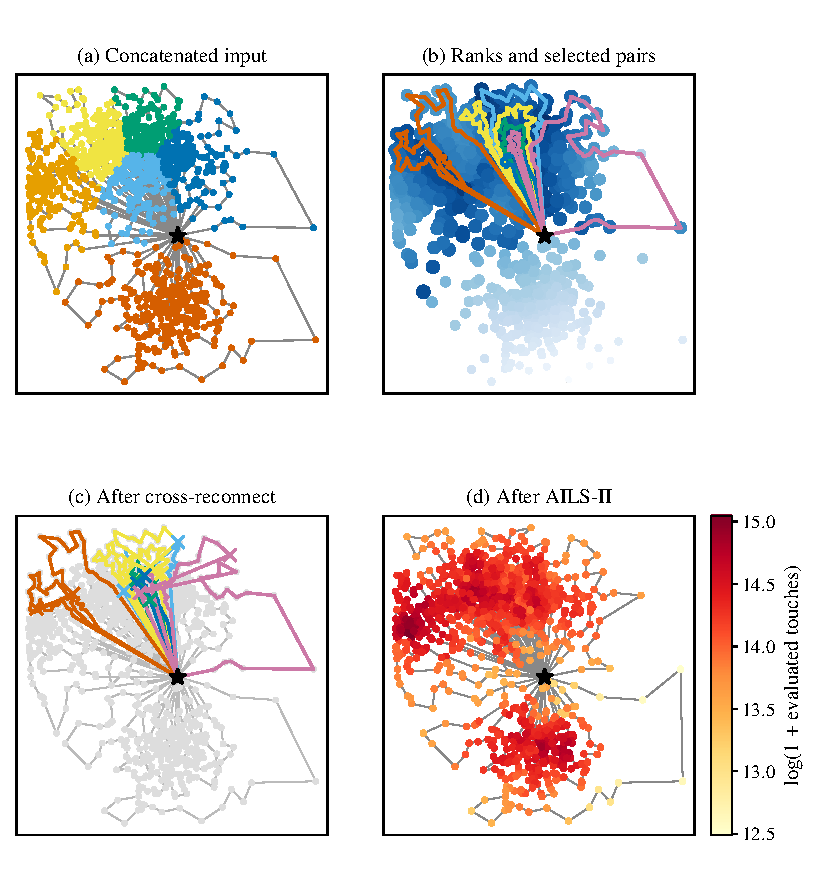
\includegraphics{figures/bgails_mechanism.pdf}
\caption[Illustrative BG-AILS Call on Instance XL-n1281-k29. Colorbar Applies to Panel (d) Only.]{Illustrative \gls{bg-ails} Call on Instance XL-n1281-k29.\\ Colorbar Applies to Panel~(d) Only.}
\label{fig:bgails-mechanism}
\end{figure}
\vspace{-\intextsep}

Table~\ref{tab:hyperparameters} lists the values of the parameters this stage introduces on top of standard AILS-II. Of these, the $\omega$ override and the boundary mask both reach into AILS-II itself. Any other AILS-II hyperparameters governing its own local search and diversification control (the parameters $d_{\min}$, $d_{\max}$, $\gamma$, and $\varphi$ of \citet{maximoHybridAdaptiveIterated2021}) are left at AILS-II's own defaults. Overriding $\omega$ to 10 against AILS-II's own starting value of 30 lowers the solver's internal perturbation degree since \gls{bg-ails} has already displaced customers across subcluster boundaries with its own cross-reconnect chain before AILS-II starts. The subsequent passes are therefore driven to intensify around that disruption rather than to add more of their own. The boundary threshold $\tau$, the small-cluster cap $\sigma$, and the boost $\alpha$ shape the ranks behind both the perturbation weights and the mask. The chain length and the pair-selection rule govern the perturbation step.

The key difference between \gls{bg-ails} and a standard AILS-II improvement pass is therefore this focus on boundary regions, imposed by the perturbation step, by the mask on the first local search, and by the short wall-clock budget \gls{bg-ails} is given. Its budget follows neither the fixed per-customer rate used for subcluster solving (Section~\ref{sec:fra-routing}) nor a plain function of instance size, but a fitted model of the surrounding decompose-route stage's own wall-clock time,
\begin{align}
\text{budget} &= \max\bigl(60\text{s},\ 1.0 \times \widehat{T}_{\mathrm{DR}}\bigr), \label{eq:bg-ails-budget}\\
\widehat{T}_{\mathrm{DR}} &= 0.976 \times n_{\mathrm{waves}}^{-0.180} \times \sum_{\text{waves}} \max(\text{per-cluster budgets in wave}), \label{eq:bg-ails-dr-wall}
\end{align}
refit on 835 pilot \gls{dri} iterations, where waves pack the current iteration's per-subcluster solver budgets (Section~\ref{sec:fra-routing}) into the granted \gls{dri} worker count in partition-submit order. The campaign of Chapter~\ref{chapter:study} runs \gls{bg-ails} asynchronously under this budget: a dedicated worker perturbs and improves the current iteration's solution while the main process decomposes and routes the next one. Section~\ref{sec:fra-pipeline} returns to Equation~\ref{eq:bg-ails-budget} as the quantity that manages the handoff.

Under this comparatively short wall-clock budget, \gls{bg-ails} should outperform an unguided AILS-II pass over the same combined solution, because the unguided pass spends an unknown and likely large share of that budget searching subcluster interiors the decomposition had already solved well. This is tested on all 100 XL instances (Section~\ref{sec:stu-dataset}) at three checkpointed decompose-route solutions each. Three different arms are forked from these checkpoints. The first control arm is a plain AILS-II pass at the solver's own defaults, the second control arm is a blind control that applies one cross-reconnect per subcluster to uniformly drawn route pairs, and the final arm is \gls{bg-ails} in its deployed configuration. Every arm receives the same AILS-II budget. The perturbation of the two perturbing arms is a surplus on top of it, an added median 0.28\% of that budget for \gls{bg-ails} and 0.010\% for the control. The checkpoints are generated under one pinned decomposition configuration, vertex K-Medoids. \gls{haos}, the route pool, and \gls{sc}/\gls{sp} are deactivated, so that the remaining comparison is one improvement stage against another on identical input, not two full runs.

\gls{bg-ails} statistically significantly outperforms both baselines (paired Wilcoxon signed-rank tests, alternative greater, Holm-corrected in a family of two). It improves on the plain AILS-II pass by 0.056~pp of cost improvement over the input solution (Hodges--Lehmann paired difference, 95\% \gls{ci} $[0.049, 0.063]$, Holm-corrected $p = 7.0 \times 10^{-11}$, ahead on 85 of 100 instances) and on the blind control by 0.058~pp (95\% \gls{ci} $[0.052, 0.065]$, Holm-corrected $p = 2.7 \times 10^{-12}$, ahead on 89 of 100). The AILS-II comparison is the practical one and carries the perturbation, the $\omega$ override, and the boundary mask as the package the framework deploys. The control comparison holds $\omega$ and chain length fixed. It measures the placement of the perturbation together with the mask: the blind arm draws its route pairs uniformly and runs AILS-II with no mask. The paired difference between the control and plain AILS-II is consistent with zero (Hodges--Lehmann $-0.004$~pp, 95\% \gls{ci} $[-0.011, 0.002]$), so the gain is not explained by perturbing the concatenated solution at all. Figure~\ref{fig:bgails-comparison} shows the arm means and the paired differences behind those tests.

\begin{figure}[H]
\centering
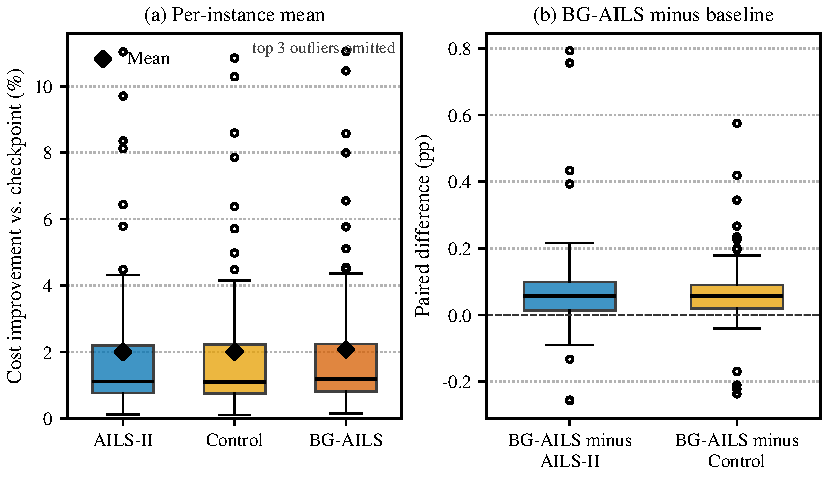
\includegraphics{figures/bgails_comparison.pdf}
\caption[Per-Instance Mean Cost Improvement (a) and Paired BG-AILS Differences (b).]{Per-Instance Mean Cost Improvement (a) and Paired \gls{bg-ails} Differences (b).}
\label{fig:bgails-comparison}
\end{figure}
\vspace{-\intextsep}

However, limiting factors apply. The comparison is only one \gls{dri} iteration, so it says nothing about what these routes are worth once the pool recombines them. It also uses a singular pinned decomposition configuration, under which the clustering and the boundary metric read the same dissimilarity matrix, as they do for three of the eight deployed clustering methods, but not for the five that cluster on raw coordinates or route centroids. And the touch counts in Figure~\ref{fig:bgails-mechanism}(d) come from a separate, identically configured instrumented run rather than from the runs the costs above are measured on.

\gls{bg-ails} finishes the \gls{dri} loop. Its output routes are contributed to the route pool like every other stage's output (Section~\ref{sec:fra-sp}), and the next iteration begins with a fresh \gls{haos} draw over the decomposition and routing operators (Section~\ref{sec:fra-haos}). At fixed intervals, \gls{drispi} recombines the routes accumulated in the pool across many \gls{dri} iterations through set covering or set partitioning, the subject of the next section.

\section[Route Pool and SC/SP Recombination]{\texorpdfstring{Route Pool and \gls{sc}/\gls{sp} Recombination}{Route Pool and SC/SP Recombination}}\label{sec:fra-sp}
Periodically, \gls{drispi} steps back from the current incumbent and recombines every route accumulated so far into one new candidate solution, using set covering or set partitioning (\gls{sc}/\gls{sp}) as the recombination model. Alternating a metaheuristic with an exact set-partitioning solve in this way is an established matheuristic pattern \citep{hybridizing_jourdan_2009}. \citet{cavaliereIntegratedLocalsearchSetpartitioning2022} apply essentially this pairing to large-scale \gls{cvrp} instances directly, by alternating LKH-3 local search with a restricted set-partitioning solve. Doing so only pays off if a shared memory of routes exists for it to recombine. So this section first describes that memory, the route pool, before turning to the \gls{sp} and \gls{sc} models themselves and the hyperparameter that decides between them.

The route pool stores one entry per distinct customer set $C_r \subseteq C$, where $C$ is the customer set of the instance (Section~\ref{sec:lit-problem}), keyed by the frozen customer set rather than by the ordered sequence of customers a route visits them in. Two routes serving the same customers in a different order, or at a different cost, are treated as the same column, and the cheaper of the two overwrites the other. This column-oriented memory, populated online during the \gls{dri} loop and periodically recombined through a partitioning model, follows the adaptive-memory principle of \citet{rochatProbabilisticDiversificationIntensification1995}, who introduce the route pool and its set-partitioning recombination for vehicle routing.

Routes are fed to the pool following a contribute-before-adopt rule, which adds a candidate solution to the pool before the pipeline decides whether to adopt it as the new incumbent, so a losing candidate still leaves its routes behind for later reuse. The \gls{dri} loop contributes to the pool twice per iteration, once from its decompose-route stage (Section~\ref{sec:fra-routing}) and once from the following improvement stage (\gls{bg-ails} (Section~\ref{sec:fra-bg-ails})). The \gls{sc}/\gls{sp} step covered in this section feeds the pool only indirectly. Solving \gls{sc} or \gls{sp} selects among the customer sets already in the pool and creates no new ones, so its own output adds nothing. Every contributed route carries a tag recording the full \gls{haos} selection that produced it, that is, $k$, the demand weight, the paradigm, the method, and the solver, with a separate flag marking routes from the post-\gls{sc}/\gls{sp} improvement pass. Whenever a candidate is adopted as the new incumbent, its routes, already in the pool by the rule above, are marked elite. Elite routes are exempt from ever being evicted from the pool to ensure the incumbent is never lost.

Every \gls{sc}/\gls{sp} solve also updates two running scores on each pool entry, A quality and a diversity score. The quality score represents a column's usefulness for the solver during the \gls{sc}/\gls{sp} solve. Therefore, an entry never touched by a solve carries no quality score yet. The diversity score is the mean Jaccard distance \citep{jaccardDistributionFloreAlpine1901} between a route's customer set and every other pool entry's customer set,
\begin{equation}
\bar{J}(r) = \frac{1}{|R| - 1} \sum_{r' \in R \setminus \{r\}} \frac{|C_r \triangle C_{r'}|}{|C_r \cup C_{r'}|},
\label{eq:route-diversity}
\end{equation}
where $R$ is the pool at the time of the update, recomputed for every entry whenever any solve happens. New quality or diversity scores are appended to a three-value window, from which final scores are read as the mean of their respective window. This ensures that single unusually high or low values do not dominate a route's standing.

These scores are a route's critical metrics when it comes to eviction from the pool. Eviction is necessary, because the route pool has a maximum size (10,000 columns by default) to keep the computational complexity of the \gls{sc}/\gls{sp} solve from blowing up. Therefore, an eviction policy is established that ranks the non-elite entries on both quality and diversity and combines their ranks into one fitness value. Among the entries that have been scored at least once, ascending order by mean quality score gives rank one to the weakest route and the highest rank to the strongest. Independently, ascending order by mean diversity score gives rank one to the most redundant route and the highest rank to the most unique. Using $\rho_q(r)$ and $\rho_d(r)$ for these two ranks, fitness is $\Phi(r) = \rho_q(r) + w_d \cdot \rho_d(r)$, with the diversity weight $w_d$ (0.5 by default) controlling how much redundancy counts against a route relative to raw quality. The entries with the lowest $\Phi(r)$ are evicted first. Because both terms grow towards the same end of their respective orderings, a route that the \gls{sc}/\gls{sp} solve relies on heavily, but that is also nearly identical to several other pool entries, can rank as a stronger eviction candidate than a weak but singular one, because redundancy drives the diversity term up regardless of quality. The eviction policy only triggers once the pool exceeds its maximum size and then only removes the overflow amount. Unscored entries are evicted only if the overflow cannot be covered by scored, non-elite entries alone.

The recombination model itself treats the pool as a column set. Let $R$ be the set of routes currently in the pool, $c_r$ the cost of route $r \in R$, that is, the Euclidean depot-customers-depot round trip over the travel costs of Section~\ref{sec:lit-problem}, and $x_r \in \{0, 1\}$ a decision variable selecting route $r$. Set partitioning, in the formulation \citet{balinskiIntegerProgramDelivery1964} introduce for exactly this delivery-routing setting, reads
\begin{align}
\text{min} \quad & \sum_{\mathclap{r \in R}} c_r x_r \label{eq:sp-obj}\\
\text{s.t.} \quad & \sum_{\mathclap{r \in R:\, i \in C_r}} x_r = 1, && \forall i \in C \label{eq:sp-partition}\\
& x_r \in \{0, 1\}, && \forall r \in R. \label{eq:sp-binary}
\end{align}
Solving Equations~\ref{eq:sp-obj}--\ref{eq:sp-binary} recombines route fragments that have never been jointly considered, for example because they may have entered the pool from different subclusters, different \gls{haos} draws, or different iterations, into one coherent solution that still covers every customer exactly once. This is the sense in which \gls{sp} looks across the boundaries any individual \gls{dri} iteration's decomposition imposes, something no individual subcluster solve or \gls{bg-ails} perturbation can do on its own.

\gls{drispi} builds this model once using Gurobi\footnote{\url{https://www.gurobi.com}} and solves it twice. It first relaxes Equation~\ref{eq:sp-binary} to the continuous $x_r \in [0, 1]$ and solves the resulting linear program. This \gls{lp} relaxation allows the solver to assign fractional weights rather than the binary ones to each route, making it significantly easier and faster to solve. The resulting fractional weights are then utilized as the quality scores fed back into the route pool above, so every \gls{sc}/\gls{sp} solve doubles as a scoring pass over the pool regardless of what it ultimately selects. This follows the same spirit in which column-generation approaches read pricing information out of \gls{lp} duals \citep{lubbeckeSelectedTopicsColumn2005}. For the second solve, the variables are then switched to binary, warm-started from the \gls{lp} solution, and re-optimized as a mixed-integer program under a wall-clock time limit and a relative optimality gap (720 seconds and 0.025\% by default). A wallclock time limit is required to cut off the search with a good, if not provably optimal, solution.

The equality constraint of Equation~\ref{eq:sp-partition} is only a meaningful choice if the pool offers more than one real alternative for most customers. A pool still dominated by a single incumbent partition would just reproduce it again and again under \gls{sp}. \gls{drispi} therefore checks, before the \gls{sc}/\gls{sp} is triggered, whether every customer in the instance is covered by at least a fixed minimum number of pool routes (five by default). Only when that holds does \gls{sp} run. Otherwise \gls{drispi} falls back to the less constrained set covering (\gls{sc}), the inequality-constrained relaxation of the same formulation \citep{garfinkelSetPartitioningProblemSetCovering1969}, whose formal problem statement and \gls{lp} relaxation are given in Appendix~\ref{app:set-covering}. \gls{sc} only requires every customer to be covered at least once rather than exactly once. Under the cover inequality a thin pool takes up a single alternative route together with the incumbent routes it overlaps, whereas the equality admits that route only once other columns fill exactly the customers it displaces. Both, \gls{sp} and \gls{sc} are safe and never blocked by infeasibility, only by a pool that has not yet accumulated enough alternatives. \gls{sc} exists to give the step something useful and always solvable to run on every scheduled trigger, warmup aside, no matter how much the pool has matured. The price of \gls{sc}'s additional permissiveness is that selected routes can overlap on a customer, meaning a customer can be visited by more than a single route and therefore more than exactly once. Since this would violate the problem statement formulated in Section~\ref{chapter:problem}, a savings-based deduplication heuristic then removes each duplicated customer from every selected route except the one where removing it would save the least cost, restoring a feasible partition.

A solved partitioning problem will pair routes into a new candidate solution which haven't been evaluated together before. And while search heuristics have been employed in identifying the routes used, the resulting new set of routes has not been polished by evaluating for example inter-route moves amongst each other. To do just that the \gls{sc}/\gls{sp} step is combined with a post-\gls{sc}/\gls{sp} improvement pass (Section~\ref{sec:fra-improve}) to improve the partitioning result even further if possible.

\section{Post-Recombination Improvement}\label{sec:fra-improve}
Once \gls{sc}/\gls{sp} (Section~\ref{sec:fra-sp}) recombines the route pool into one partition, \gls{drispi} runs one further pass over it using AILS-II as solver, seeded only with that partition as an initial solution. Unlike in \gls{bg-ails} (Section~\ref{sec:fra-bg-ails}), this step focuses less on perturbation but rather refinement by local search. This post-recombination improvement pass also allows the solver to touch all routes instead of guiding moves towards certain neighborhoods. The pass runs under its own wall-clock budget (360 seconds by default) on the same core reservation as the \gls{sc}/\gls{sp} solve that precedes it. Section~\ref{sec:fra-pipeline} elaborates how exactly a parallel architecture of \gls{drispi} looks.

The refined routes feed back into the route pool exactly like every other stage's output (see Section~\ref{sec:fra-sp}). A route whose customer set matches one \gls{sc}/\gls{sp} already selected keeps that route's existing tag, while a route created by moving customers between routes in this stage is added as new, and tagged as an improvement route rather than credited to an existing \gls{haos} selection.

This is also where the deferred rewards of \gls{haos} are distributed (Section~\ref{sec:fra-haos}). The pass's outcome, a new best, an improvement over the previous iteration without beating the incumbent, or neither, is scored through the deferred branch of \gls{haos}'s reward function and credited not to the current iteration's own draw but to every distinct \gls{haos} tag the routes \gls{sc}/\gls{sp} selected already carried. That is, to whichever earlier decompose-route or \gls{bg-ails} draws produced those specific routes, regardless of how many iterations ago that was. Improvement-route tags are excluded from this credit, since this stage created them without any \gls{haos} draw of their own to reward.

\section{Parallelized Pipeline Orchestration}\label{sec:fra-pipeline}
The preceding sections describe \gls{haos}, decomposition, routing, \gls{bg-ails}, the route pool and \gls{sc}/\gls{sp}, and the post-\gls{sc}/\gls{sp} improvement pass as if they were executed sequentially, like Figure~\ref{fig:dri-overview} shows. And while \gls{drispi}'s implementation allows for sequential execution, it also offers a more potent, highly parallelized mode as well. For that it splits eight cores into three disjoint groups and distributes six for the main loop and the \gls{dri} routing pool of Section~\ref{sec:fra-routing}, one for the \gls{bg-ails} worker of Section~\ref{sec:fra-bg-ails}, and one for the \gls{sc}/\gls{sp} and post-\gls{sc}/\gls{sp} improvement worker of Sections~\ref{sec:fra-sp} and~\ref{sec:fra-improve}. A main orchestration process shares the six \gls{dri} cores rather than occupying a ninth.

Figure~\ref{fig:pipeline-swimlane} shows what this asynchronous, parallelized mode looks like across two consecutive iterations. After decompose-route of iteration~$i$ the loop waits for job~$i{-}1$ and drains it~\mk{1}, then launches job~$i$ on the new solution~\mk{2}. After decompose-route of iteration~$i{+}1$ the same pair of steps waits for job~$i$, drains it, and launches job~$i{+}1$. A finished \gls{sc}/\gls{sp} job is drained without blocking~\mk{3} at the start of the following iteration.

\begin{figure}[tbp]
\centering
\resizebox{\linewidth}{!}{% ---------------------------------------------------------------------------
% DRISPI parallelized pipeline, iterations i and i+1 (schematic).
% Requires: arrows.meta, patterns, decorations.pathreplacing, calc
% Block lengths are illustrative; the order of events follows the main loop.
% ---------------------------------------------------------------------------
\begin{tikzpicture}[
  font=\small\normalfont,
  >={Latex[length=1.8mm]},
  blk/.style={draw, thick, minimum height=0.8cm, inner sep=1pt, anchor=west,
              align=center, font=\footnotesize},
  dr/.style={blk, fill=blue!12},
  hs/.style={blk, fill=blue!30!black!80, text=white, font=\scriptsize\normalfont\bfseries},
  bg/.style={blk, fill=orange!18},
  wait/.style={draw, thick, pattern=north east lines, pattern color=black!45,
               minimum height=0.8cm, inner sep=0pt, anchor=west},
  launch/.style={->, thick},
  drain/.style={->, thick, dashed},
  num/.style={circle, draw, thick, fill=white, inner sep=0.6pt,
              font=\scriptsize\bfseries, minimum size=3.6mm},
  lbl/.style={font=\scriptsize},
]
\def\yD{0}\def\yB{-1.4}\def\yS{-2.8}
\def\h{0.4}
\def\pblk#1#2#3#4#5{\node[#1, minimum width=#4cm-#3cm] at (#3,#2) {#5};}

% ---- lanes -----------------------------------------------------------------
\foreach \y/\n/\c in {\yD/DRI-Loop/6 cores, \yB/BG-AILS/1 core, \yS/SP/1 core}{
  \node[anchor=east, align=right] at (-0.35,\y) {\n\\[-1pt]{\scriptsize (\c)}};
  \draw[black!20] (-0.2,\y) -- (11.6,\y);
}

% ---- iteration brackets ------------------------------------------------------
\draw[decorate, decoration={brace, amplitude=5pt}, thick]
  (0,\yD+\h+0.12) -- node[above=5pt] {iteration $i$} (5.7,\yD+\h+0.12);
\draw[decorate, decoration={brace, amplitude=5pt}, thick]
  (5.8,\yD+\h+0.12) -- node[above=5pt] {iteration $i{+}1$} (11.0,\yD+\h+0.12);

% ---- DRI-Loop --------------------------------------------------------------
\pblk{hs}{\yD}{0}{0.35}{H}
\pblk{dr}{\yD}{0.35}{4.8}{decompose\,+\,route $i$}
\node[wait, minimum width=0.6cm] at (4.8,\yD) {};
\pblk{hs}{\yD}{6.2}{6.55}{H}
\pblk{dr}{\yD}{6.55}{10.8}{decompose\,+\,route $i{+}1$}

% ---- bg --------------------------------------------------------------------
% BG-AILS i-1 was launched at the end of iteration i-1 (open left edge)
\fill[orange!18] (-0.2,\yB-\h) rectangle (5.4,\yB+\h);
\draw[thick] (-0.2,\yB-\h) -- (5.4,\yB-\h) -- (5.4,\yB+\h) -- (-0.2,\yB+\h);
\node[font=\footnotesize] at (2.7,\yB) {BG-AILS $i{-}1$};
\pblk{bg}{\yB}{5.6}{9.9}{BG-AILS $i$}
\node[lbl, text=black!60] at (10.35,\yB) {idle};
\fill[orange!18] (11.0,\yB-\h) rectangle (11.6,\yB+\h);
\draw[thick] (11.6,\yB-\h) -- (11.0,\yB-\h) -- (11.0,\yB+\h) -- (11.6,\yB+\h);
\node[font=\footnotesize] at (11.3,\yB) {$i{+}1$};

% ---- sp --------------------------------------------------------------------
% SC/SP job dispatched at an earlier trigger (open left edge)
\fill[black!8] (-0.2,\yS-\h) rectangle (3.4,\yS+\h);
\draw[thick] (-0.2,\yS-\h) -- (3.4,\yS-\h) -- (3.4,\yS+\h) -- (-0.2,\yS+\h);
\node[font=\footnotesize] at (1.6,\yS) {SC/SP\,+\,AILS-II};
\node[lbl, text=black!60, anchor=west] at (3.55,\yS) {done};
\node[lbl, text=black!60, anchor=west] at (6.55,\yS) {idle until the next trigger};

% ---- handoffs ----------------------------------------------------------------
% end of iteration i: wait for BG i-1, drain it, launch BG i
\draw[drain]  (5.4,\yB+\h) -- (5.4,\yD-\h);
\draw[launch] (5.6,\yD-\h) -- (5.6,\yB+\h);
\node[num] at (5.12,-0.7) {1};
\node[num] at (5.83,-0.7) {2};
% start of iteration i+1: drain the finished SC/SP job (non-blocking)
\draw[white, line width=3.5pt] (6.12,\yB-\h) -- (6.12,\yB+\h);
\fill (6.12,\yS) circle (1.5pt); \draw[drain] (6.12,\yS) -- (6.12,\yD-\h);
\node[num] at (6.4,-2.1) {3};
% end of iteration i+1: BG i already finished, no wait
\draw[drain]  (10.8,\yB+\h) -- (10.8,\yD-\h);
\draw[launch] (11.0,\yD-\h) -- (11.0,\yB+\h);
\node[num] at (10.52,-0.7) {1};
\node[num] at (11.28,-0.7) {2};

% ---- one-iteration lag -------------------------------------------------------
\draw[decorate, decoration={brace, amplitude=4pt, mirror}, thick]
  (6.55,\yD-\h-0.1) -- node[lbl, below=4pt, fill=white, inner sep=1pt] {runs alongside BG-AILS $i$} (9.9,\yD-\h-0.1);

% ---- legend ----------------------------------------------------------------
\begin{scope}[shift={(0,-3.85)}, every node/.style={lbl, anchor=west}]
  \node[num, anchor=center] at (0.15,0)     {1}; \node at (0.35,0)     {wait for the previous BG-AILS job and drain it};
  \node[num, anchor=center] at (0.15,-0.45) {2}; \node at (0.35,-0.45) {launch BG-AILS on the new solution};
  \node[num, anchor=center] at (0.15,-0.9)  {3}; \node at (0.35,-0.9)  {drain a finished SC/SP job (non-blocking)};
  \node[hs, anchor=center, minimum height=3.6mm, minimum width=3.6mm] at (7.0,0) {H};
  \node at (7.2,0) {HAOS draw};
  \node[wait, anchor=center, minimum width=3.6mm, minimum height=3.6mm] at (7.0,-0.45) {};
  \node at (7.2,-0.45) {main loop blocked};
\end{scope}
\end{tikzpicture}
}
\caption[Two Consecutive DRISPI Iterations in One 8-Core Container (6 for DRI, 1 for BG-AILS, and 1 for SP). Block Lengths Are Illustrative.]{Two Consecutive \gls{drispi} Iterations in One 8-Core Container 
(6 for \gls{dri}, 1 for \gls{bg-ails}, and 1 for \gls{sp}). Block Lengths Are Illustrative.}
\label{fig:pipeline-swimlane}
\end{figure}

Equation~\ref{eq:bg-ails-budget} sizes the \gls{bg-ails} budget to the decompose-route stage it overlaps with, which is what keeps the wait at~\mk{1} short. A budget much shorter than the next decompose-route pass would leave the \gls{bg-ails} core idle before the handoff. A budget much longer would leave the \gls{dri} cores blocked on a job that already had the next iteration's input ready. In Figure~\ref{fig:pipeline-swimlane} the wait after decompose-route of iteration~$i{+}1$ vanishes because job~$i$ finished during that pass.

The \gls{sc}/\gls{sp} worker uses a skip policy rather than a blocking handoff. The campaign checks the trigger only at iteration boundaries, so a job starts at the first boundary after the x-minute mark (20 by default), not exactly at it. \gls{drispi} then dispatches a snapshot of the route pool and the incumbent only if the worker is idle. If it is busy, the trigger is skipped rather than queued. The worker owns both the \gls{sc}/\gls{sp} solve and the post-\gls{sc}/\gls{sp} improvement pass of Section~\ref{sec:fra-improve}, running them one after another on the same core. Those two default ceilings, 720~s and 360~s, sum to 18 minutes and therefore leave two minutes of slack under the default 20-minute interval. A skip is therefore only necessary if enqueue and overhead consume that slack.

Algorithm~\ref{alg:pipeline} shows the complete and deployed \gls{drispi} loop. After decompose-route the loop waits for the previous \gls{bg-ails} job~\mk{1}, drains it through Absorb, and launches the next job on $(S_{\mathrm{DR}}, \kappa, \lambda_q)$~\mk{2}, keeping $\theta$ only for later credit. A finished \gls{sc}/\gls{sp} job is absorbed without blocking~\mk{3} at the start of the next iteration. A synchronous mode that runs both stages inline is implemented as a code option and recovers the sequential picture of Figure~\ref{fig:dri-overview}.

\begin{algorithm}[tbp]
\caption{\gls{drispi} Main Loop as Deployed (Async. \gls{bg-ails} and \gls{sp})}\label{alg:drispi}\label{alg:pipeline}
\KwIn{instance; time limit $\Gamma$}
\KwInit{$R \gets \emptyset$; $S^\star$ undefined; $i \gets 0$}
\BlankLine
\While{elapsed time $< \Gamma$}{
  \If{the \gls{sc}/\gls{sp} job has finished}{
    \Absorb{$S_{\mathrm{\gls{sp}}}, \Theta_{\mathrm{\gls{sp}}}$, deferred} \tcp*[r]{$\Theta_{\mathrm{\gls{sp}}}$: tags of selected routes}
  }
  $(\theta, \text{config}) \gets \Draw{$S^\star$}$ \tcp*[r]{Algorithm~\ref{alg:haos}}
  decompose into $k$ subclusters under config \tcp*[r]{Section~\ref{sec:fra-decomposition}}
  \ParFor{each subcluster}{route it with the drawn solver \tcp*[r]{Section~\ref{sec:fra-routing}}}
  $S_{\mathrm{DR}} \gets$ concatenated subcluster routes; \Absorb{$S_{\mathrm{DR}}, \{\theta\}$, immediate}\;
  \If{a \gls{bg-ails} job is in flight}{
    wait for its result $(S_{\mathrm{BG}}, \theta')$; \Absorb{$S_{\mathrm{BG}}, \{\theta'\}$, immediate}\;
  }
  dispatch \gls{bg-ails} on $(S_{\mathrm{DR}}, \kappa, \lambda_q)$ \tcp*[r]{Algorithm~\ref{alg:bgails}; $\theta$ for credit}
  \If{\gls{sc}/\gls{sp} is due \KwAnd the sp worker is idle}{
    dispatch \SPJob{$R, S^\star$} to the sp worker\;
  }
  \Decay{}; $i \gets i + 1$\;
}
\Return $S^\star$\;
\BlankLine
\Fn{\Absorb{$S, \Theta$, channel}}{
  $r \gets$ reward of $S$ in this channel (Table~\ref{tab:haos-rewards})\;
  add the routes of $S$ to $R$; \lIf{$c(S) < c(S^\star)$}{$S^\star \gets S$}
  \lForEach{$\theta \in \Theta$}{\Credit{$\theta, r$}}
}
\BlankLine
\Fn{\SPJob{$R, S^\star$}}{
  \leIf{min.\ coverage of $R \geq 5$}{$S \gets \mathrm{\gls{sp}}(R)$}{$S \gets \mathrm{dedup}(\mathrm{\gls{sc}}(R))$}
  \Return $\solver(S)$ under the improvement budget \tcp*[r]{Section~\ref{sec:fra-improve}}
}
\end{algorithm}

This Algorithm~\ref{alg:pipeline} is the loop the following Chapter~\ref{chapter:study} evaluates. It is run, unchanged, on all 100 XL instances under a two-hour budget, and the resulting costs are compared with the monolithic solvers benchmarked on that set.
\chapter{Computational Study}\label{chapter:study}
This chapter tests \gls{drispi} on the 100 XL instances of Queiroga et al.\ (2026)
against the eight monolithic solvers benchmarked there. The study aims to answer two questions:
The first is whether an adaptive decomposition framework that learns its
decomposition and routing choices during a run can match state-of-the-art
monolithic solvers at this scale. The second is whether the weights HAOS learns along the way provide interpretable 
insights about the instances they were learned on.

Section~\ref{sec:stu-experiment} describes the dataset, specifies implementation and
hardware specificiations, the parameter values, and explains expertimental design choices. Section~\ref{sec:stu-results} shows and analyzes the results. Here we answer the primary and secondary research questions through comparison with the published solvers, breaks the results down by instance characteristics, and examines the learned HAOS weights and the convergence of
individual runs.

\section{Experimental Design}\label{sec:stu-experiment}
All 100 instances are solved by the same \gls{drispi} configuration. Nothing is tuned
per instance by design without anyexceptions. Section~\ref{sec:stu-dataset} describes the instances and the reference solutions used as baseline, section~\ref{sec:stu-implementation} the software and hardware the campaign
ran on, section~\ref{sec:stu-hyperparameters} the parameter values, and
section~\ref{sec:stu-repetitions} the number of seeds and the statistical precision it buys for our experiment.

\subsection{Dataset}\label{sec:stu-dataset}
The XL set (section~\ref{sec:lit-problem}) extends the generation scheme of the X
instances of \citet{uchoaNewBenchmarkInstances2017} to up to 10,000 customers. Every instance
places its nodes on a $[0, 1000] \times [0, 1000]$ grid with Euclidean distances
and combines one level of each of four attributes. The depot is Random, Central
at $(500, 500)$, or Eccentric at $(0, 0)$ in the bottom left corner. Customers are Random, Clustered, or
Random-Clustered around a small number of seed points. Demand follows one of
seven distributions: unitary (U), four ranges of increasing width (1--10, 5--10,
1--100, 50--100), a quadrant-dependent range (Q), or many small and few large
demands (SL). The target average route length $r$ lies in one of seven bands,
from ultra-short ($r \in [3, 5]$) to ultra-long ($r \in [50, 200]$), and
capacity $Q$ is set so that a solution with the minimum number of routes attains
it. The instance name references $n$ and that minimum route count, e.g.\
XL-n4535-k1134. This $k$ equals $\lceil \sum_{i=1}^{n} q_i / Q \rceil$, making it the mathematical minimum number of routes, because fewer vehicles could not carry the total customer demand under capacity set to $Q$. This $k$ is
fixed by the benchmark and unrelated to the subcluster count $k$ of Section~\ref{sec:fra-haos}.
Table~\ref{tab:xl-summary} breaks down the above mentioned characteristics on a per-instance basis along with \gls{drispi}'s result and comparison to initial and current \gls{bks} values.

The initial BKS values of \citet{queirogaXLInstancesCapacitated2026} come from the solver
runs described in section~\ref{sec:lit-large-cvrp} and were released as baselines with the
CVRPLib BKS Challenge, a community competition opened on January~12, 2026, in
which any team can submit an improved solution for automatic verification. By
the current record,\footnote{\url{https://galgos.inf.puc-rio.br/cvrplib/index.php/en/bks_challenge/score/instances}, accessed September 7, 2026.} the challenge has improved 99 of the 100
initial values, leaving only XL-n1094-k157 to still hold its initial value. We report the
percentage gap to baselines such as the initial and the current \gls{bks}:
\begin{equation}
\mathrm{Gap} = 100 \times \frac{c - c_{\mathrm{BKS}}}{c_{\mathrm{BKS}}}.
\label{eq:gap}
\end{equation}
The quantity $c$ is the reported solution cost. The current
\gls{bks} represents the official best known solution. However, we primarily compare against initial \gls{bks}, because published solvers produced it in two-hour single-thread runs on specified hardware
(Section~\ref{sec:lit-large-cvrp}), using us an experimental design we can reproduce to allow for any algorithmic comparability. The official BKS values on the other hand have been achieved without constraints regarding computational, with many of them coming from day-long runs that rely on raw compute, rendering any fair comparison infeasible.

\subsection{Framework Implementation}\label{sec:stu-implementation}
All experiments in this chapter run on a single, shared department server under
Ubuntu 22.04.5 LTS with two Intel Xeon Platinum~8280L CPUs at 2.70\,GHz
(28 cores each, 56 cores and 112 threads total) and 5,928\,GiB of RAM, with no
GPU\@. \gls{drispi} runs inside Docker containers (Docker 28.1.1) pinned to a disjoint physical-core range with \texttt{--cpuset-cpus}. This pinned CPU count, not a library thread-pool default, sets the framework's parallelism budget.

The campaign presented in section~\ref{sec:stu-comparison} is comprised of all 100 instances, each run on three seeds with a wallclock runtime budget and termination criterion of T=2h (300 runs, 7{,}200 seconds each). For that we pin 48 of the server's 56 physical cores as six exclusive 8-core Docker containers, three per socket, parallelizing as outlined in section~\ref{sec:fra-pipeline} with a split into six DRI workers, one BG-AILS worker, and one SP worker. SMT siblings are left idle. Runs are packed into waves ordered by instance size so that the three seeds of the largest instance, XL-n10001-k1570, never share a wave. The full campaign takes 50 waves and about 100 hours of wall-clock time.

\gls{drispi} uses Python 3.11, with dependencies locked via \texttt{uv}: Libraries PyVRP 0.13.3 (HGS-CVRP), scikit-learn 1.8.0 (K-Means and Agglomerative Clustering), scikit-learn-extra 0.3.0 (K-Medoids), scikit-fuzzy 0.5.0 (Fuzzy C-Means), gurobipy 13.0.1 (SC/SP), and vrplib 2.1.0 for instance parsing. AILS-II, FILO, and FILO2 are vendored as git submodules pinned to a fixed commit each and compiled at image build time, rather than resolved from a floating branch, so a rebuild reproduces the exact binaries behind the results in Section~\ref{sec:stu-comparison}. The whole framework runs inside a Docker image built from this locked environment, so the software stack behind every reported run is fixed independently of the host it executes on.

\subsection{Hyperparameters}\label{sec:stu-hyperparameters}
\begin{table}[!htb]
\centering\small
\caption{Hyperparameters of the Benchmark Configuration.}
\label{tab:hyperparameters}
\begin{tabular}{@{}lll@{}}
\toprule
Parameter & Value & Defined in \\
\midrule
\multicolumn{3}{@{}l}{\emph{HAOS}} \\
Warm-up iterations & 10 & Section~\ref{sec:fra-haos} \\
Decay $\gamma$ & 0.95 & Equation~\ref{eq:haos-decay} \\
Starting weight $w_0$ & 10.0 & Equation~\ref{eq:haos-update} \\
Floor $p_{\min}$: $k$ / $\lambda_q$, method, solver / paradigm & 0.025 / 0.05 / 0.10 & Equation~\ref{eq:haos-probability} \\
Immediate and deferred rewards & Table~\ref{tab:haos-rewards} & Section~\ref{sec:fra-haos} \\
\addlinespace
\multicolumn{3}{@{}l}{\emph{Decomposition and routing}} \\
Base $k$ arms & $\{2,3,4,6,8,10,12\}$ & Section~\ref{sec:fra-haos} \\
Maximum number of $k$ arms & 10 & Section~\ref{sec:fra-haos} \\
Minimum routes per subcluster & 8 & Section~\ref{sec:fra-haos} \\
Minimum spacing between $k$ arms & 2 & Section~\ref{sec:fra-haos} \\
Subcluster time budget & $\max(5\,\mathrm{s},\ 0.06\,\mathrm{s} \cdot n_c)$ & Section~\ref{sec:fra-routing} \\
\addlinespace
\multicolumn{3}{@{}l}{\emph{BG-AILS}} \\
Boundary threshold $\tau$ & 0.5 & Equation~\ref{eq:bg-ails-threshold} \\
Small-cluster cap $\sigma$ / boost $\alpha$ & 20 / 0.5 & Equation~\ref{eq:bg-ails-weighted} \\
Initial $\omega_0$ & 10 & Section~\ref{sec:fra-bg-ails} \\
First-route selection & greedy, unique first & Section~\ref{sec:fra-bg-ails} \\
Chain length & $k$ & Section~\ref{sec:fra-bg-ails} \\
Boundary mask on first local search & on & Section~\ref{sec:fra-bg-ails} \\
Budget floor / margin & 60\,s / 1.0 & Equation~\ref{eq:bg-ails-budget} \\
\addlinespace
\multicolumn{3}{@{}l}{\emph{Route pool, SC/SP, and improvement}} \\
Maximum pool size & 10{,}000 & Section~\ref{sec:fra-sp} \\
Diversity weight $w_d$ & 0.5 & Section~\ref{sec:fra-sp} \\
SC/SP trigger interval & 20\,min & Section~\ref{sec:fra-pipeline} \\
Minimum coverage for SP & 5 & Section~\ref{sec:fra-sp} \\
MIP time limit / relative gap & 720\,s / 0.025\,\% & Section~\ref{sec:fra-sp} \\
Improvement pass time limit & 360\,s & Section~\ref{sec:fra-improve} \\
\bottomrule
\end{tabular}
\end{table}
Table~\ref{tab:hyperparameters} lists the parameter values of the benchmark
configuration, which all 100 instances and all three seeds share.
Chapter~\ref{chapter:framework} introduces each parameter with its mechanism, the
table collects the values used to achieve the results presented in section~\ref{sec:stu-results}.
Most parameters were tuned during development in isolated pilot studies per category (HAOS, Decomposition and Routing, BG-AILS, Route Pool, SC/SP, and Improvement). These small studies were comprised of a few instances and seeds, usually running a limited parameter grid search, aimed at finding a reasonable default rather than an optimum, and these studies are not reported here. The only exception is the BG-AILS comparison of Section~\ref{sec:fra-bg-ails}, which ran on all 100 XL
instances and fixed the first-route rule and the boundary mask; these two
settings are therefore chosen on the benchmark set itself. No sensitivity
analysis over the full set was run for any of the other values.

Not included in the table are the option sets HAOS draws from: the number of subclusters $k$, the six values of $\lambda_q$, the two paradigms, the eight clustering methods of Table~\ref{tab:decomp-methods}, and the four
routing solvers of Section~\ref{sec:fra-routing}. They define the search space of
HAOS rather than a value within it. Also excluded are settings regarding the campaign architecture and experimental design: the core split and asynchronous modes of Section~\ref{sec:fra-pipeline}, the fitted coefficients of the
BG-AILS wall-time model (Equation~\ref{eq:bg-ails-dr-wall}), and the time limit and seeds that Section~\ref{sec:stu-repetitions} covers.

\subsection{Replication Design}\label{sec:stu-repetitions}
The campaign runs \gls{drispi} on every one of the 100 XL instances three times, at
seeds 11, 22, and 33. The seed drives the weighted HAOS draws, the angular
offset, and the random choices inside decomposition. It is also
passed to PyVRP, FILO, and FILO2, but AILS-II has no seed flag. This makes the routing phase, BG-AILS and the post-SC/SP improvement pass independent of the seed. This makes the runs non-reproducible. Additionally, the plugged-in solvers run under wall-clock limits, so how far their search gets depends on machine load, and the worker pool
schedules subcluster jobs in no fixed order. This affects again, the entire routing phase,
BG-AILS, and the post-SC/SP improvement pass alike, so two runs at the same seed
can differ in solution quality. Disclosing the seeds therefore does not suffice
for exact reproducibility. The three runs per instance are exchangeable replications.

Because each run is stopped after 7,200 seconds (120 minutes) of wall-clock time rather than at convergence, each run resembles a terminating simulation in the sense of \citet{lawSimulationModelingAnalysis2000}: a fixed initial condition, the first DRI iteration's decomposition and routing pass (Section~\ref{sec:fra-decomposition}), and a fixed stopping rule rather than a steady state. The replication method of \citet[ch.~9]{lawSimulationModelingAnalysis2000} therefore applies.

The precision target refers to the fixed set of 100 instances, which are a design
factor \citep{queirogaXLInstancesCapacitated2026} rather than a sample from a larger
population, so the seed is the only randomness the design controls. Using
$\bar G$ the grand mean gap and $\bar\sigma^2$ the average per-instance seed
variance, we get $\mathrm{Var}(\bar G) = \bar\sigma^2 / (I \cdot S)$ with
$I = 100$. The $I \cdot S$ observations are independent by construction. Every
run is a separate process with its own random-number stream, and no pool, cache,
or counter is shared across runs (Chapter~\ref{chapter:framework}). This interval does
not extend to the published baselines of Section~\ref{sec:stu-comparison}, which
report one value per instance and no variance.

A pilot campaign of three diverse instances with four seeds each measured a
root-mean-square per-instance seed standard deviation of 0.118\,pp at the
7{,}200-second mark. The target half-width was fixed in advance at 0.03\,pp, small
enough to resolve the 0.02--0.06\,pp effects seen in earlier component tests.
Table~\ref{tab:seed-sizing} forecasts the standard error and the 95\%
half-width of $\bar G$ at the pilot value. Every $S$ from one to four meets the
target. This would in fact still hold true at a 99\% interval, but precision alone does not decide $S$.

\begin{table}[htbp]
\centering
\caption{Forecast Standard Error and 95\% Half-Width of $\bar G$ by Seed Count $S$.}\label{tab:seed-sizing}
\begin{tabular}{@{}lrr@{}}
\toprule
$S$ & SE (pp) & Half-width (pp) \\
\midrule
1 & 0.0118 & 0.023 \\
2 & 0.0083 & 0.016 \\
3 & 0.0068 & 0.013 \\
4 & 0.0059 & 0.012 \\
\bottomrule
\end{tabular}
\end{table}

Three other considerations set $S = 3$. At $S = 1$ there are no within-instance
degrees of freedom and no interval at all. At $S = 2$ a discrepancy between two
runs is visible, but cannot be attributed to either of them. At $S = 3$, however, one
anomalous run stands out against the other two. We also require $S > 1$ to present a best-of-$S$ column, which is the
convention on this instance set \citep{queirogaXLInstancesCapacitated2026}.

A fourth seed would add 100 runs and 1,600 core-hours to shrink the half-width
from 0.013 to 0.012\,pp. That gain is too small next to a second source of error.
Two pilot campaigns that differed only in execution environment produced means
0.039\,pp apart, three times the $S = 3$ half-width. Such a batch effect shifts
every run of a campaign alike, so more seeds do not reduce it, and the budget of
a fourth seed would not buy a meaningfully more precise $\bar{G}$
\citep{barrDesigningReportingComputational1995,johnsonTheoreticiansGuideExperimental2002}.
Neyman allocation, which assigns seeds in proportion to each instance's standard
deviation \citep{neymanTwoDifferentAspects1934,cochranSamplingTechniques1977}, would have further complicated the experimental design while only cutting the standard error of $\bar{G}$ by 8.8\% at the same total budget. Therefore, every instance receives
three seeds.

The pilot value was conservative. In the campaign, the mean per-instance seed
standard deviation is 0.035\,pp % TODO: report the RMS value, which is what enters Var(G)
(Section~\ref{sec:stu-comparison}), about a third of the pilot value,
which puts the realized 95\% half-width of $\bar G$ near 0.004\,pp. This
interval applies to the mean over seeds only. Best-of-$S$ is an extreme-value
statistic whose expectation depends on $S$, so it is not comparable across
studies with different replication counts. Section~\ref{sec:stu-comparison} uses
it descriptively and focuses its main comparison and the answer to our primary research questions on the mean-of-$S$ gap.

\section{Results}\label{sec:stu-results}
Short introduction.
% Need to define how exactly I am going to answer RQs here. Suggestion: We are competitive if we are not significantly worse than the SOTA Solvers. This will hold up for more 7/8 and give it the right spin I believe.

\subsection{Performance Comparison against State-of-the-Art Monolithic Solvers}\label{sec:stu-comparison}
Table~\ref{tab:solver-summary} compares \gls{drispi} against the eight monolithic solvers \citet{queirogaXLInstancesCapacitated2026} benchmark on the 100 XL instances: AILS-II, FILO, FILO2, KGLSXXL, HGS-CVRP, SISRs, LKH-3, and OR-Tools. For every solver we recompute the percentage gap to the current official \gls{bks}, the record listed by the CVRPLib \gls{bks} Challenge (Section~\ref{sec:stu-dataset}), for both the mean-of-$N$ and best-of-$N$ cost the original paper reports ($N=60$ for the published solvers, $N=3$ for \gls{drispi}), then average that per-instance gap over all 100 instances and, separately, over the fifty instances with fewer than 3,400 customers and the fifty with more, the split \citet{queirogaXLInstancesCapacitated2026} use for their own results table. Every gap in Table~\ref{tab:solver-summary} uses the current \gls{bks} as the denominator, including for the published solvers. \citet{queirogaXLInstancesCapacitated2026} report their own average gaps against the \gls{bks} at the time of publication, effectively AILS-II's own result for most instances, so those published averages are not comparable to the ones reported here. Appendix~\ref{app:xl-results} lists the per-instance detail behind \gls{drispi}'s two columns: instance characteristics, best cost, and gap, alongside both \gls{bks} references (Table~\ref{tab:xl-summary}).

Table~\ref{tab:solver-summary} sets \gls{drispi}'s runs against the published solvers under
different hardware and budgets. \gls{drispi} runs 7,200 seconds of wall-clock time per
instance and seed on eight pinned cores (Section~\ref{sec:stu-implementation});
\citet{queirogaXLInstancesCapacitated2026} ran every published solver on a single thread of
two AMD EPYC~9654 processors, 60 seeds of two hours per instance.
Section~\ref{sec:con-limitations} discusses what this difference means for
the two columns of the table.

\begin{longtable}{@{}lrrrrrr@{}}
\caption{\gls{drispi} Mean Gap to Current \gls{bks} Comparison Against Benchmark  Solvers, Sorted by Ascending Mean-of-$N$ Gap Over All Instances.}\label{tab:solver-summary}\\
\toprule
& \multicolumn{3}{c}{Mean-of-$N$ Gap (\%)} & \multicolumn{3}{c}{Best-of-$N$ Gap (\%)} \\
\cmidrule(lr){2-4} \cmidrule(lr){5-7}
Solver & All & $n<3{,}400$ & $n>3{,}400$ & All & $n<3{,}400$ & $n>3{,}400$ \\
\midrule
\endfirsthead
\toprule
& \multicolumn{3}{c}{Mean-of-$N$ Gap (\%)} & \multicolumn{3}{c}{Best-of-$N$ Gap (\%)} \\
\cmidrule(lr){2-4} \cmidrule(lr){5-7}
Solver & All & $n<3{,}400$ & $n>3{,}400$ & All & $n<3{,}400$ & $n>3{,}400$ \\
\midrule
\endhead
\bottomrule
\endfoot
\bottomrule
\endlastfoot
AILS-II & +0.16 & +0.14 & +0.18 & +0.09 & +0.06 & +0.12 \\
FILO2 & +0.29 & +0.29 & +0.30 & +0.20 & +0.17 & +0.23 \\
\gls{drispi} & +0.31 & +0.24 & +0.37 & +0.28 & +0.21 & +0.34 \\
FILO & +0.33 & +0.31 & +0.36 & +0.24 & +0.19 & +0.28 \\
SISRs & +0.58 & +0.49 & +0.68 & +0.42 & +0.30 & +0.55 \\
KGLSXXL & +1.09 & +0.87 & +1.31 & +0.88 & +0.64 & +1.12 \\
HGS-CVRP & +1.45 & +0.83 & +2.06 & +1.20 & +0.60 & +1.80 \\
LKH-3 ($n = 90$) & +6.75 & +5.01 & +8.92 & +5.56 & +4.03 & +7.48 \\
OR-Tools & +6.90 & +6.77 & +7.03 & +5.63 & +5.43 & +5.83 \\

\end{longtable}

Mean-of-$N$ is the primary comparison in Table~\ref{tab:solver-summary}, because \gls{drispi}'s mean-of-3 and each published solver's mean-of-60 both estimate the same population quantity, the expected cost of a single run, and are just averages over different sample sizes. Best-of-$N$ is not: it is the minimum of three draws for \gls{drispi} against the minimum of sixty for every published solver, a sampling budget 20 times larger, which mechanically favors the columns with more draws. Sampling one of \gls{drispi}'s own three seed costs at a time gives an expected best-of-1 gap equal to the mean-of-3 gap, 0.309\%; the average of the smaller cost in each of the three retained seed pairs gives a best-of-2 gap of 0.286\%; the actual three-seed minimum gives the best-of-3 gap of 0.277\%, already reported in Table~\ref{tab:solver-summary}. The marginal gain is 0.022 pp from the first extra sample and 0.009 pp from the second. AILS-II, FILO2, FILO, SISRs, KGLSXXL, and HGS-CVRP gain 0.07, 0.09, 0.10, 0.16, 0.21, and 0.25 pp respectively between their own mean-of-60 and best-of-60 columns, larger reductions from many more repetitions. \gls{drispi}'s mean per-instance seed standard deviation is 0.035 pp, so additional seeds narrow its best column by less than they narrow a higher-variance baseline's. This produces the rank inversion in Table~\ref{tab:solver-summary}: \gls{drispi} ranks third by mean-of-$N$ and fourth by best-of-$N$, without a change in the underlying solution quality; the difference is which column rewards low run-to-run variance and which rewards a wide sampling budget. Best-of-$N$ is reported to match the published solvers' own headline metric, not as the primary comparison.

The means in Table~\ref{tab:solver-summary} do not establish whether an observed difference is real rather than an artifact of the 100 sampled instances. We tested \gls{drispi}'s mean-of-3 column against the corresponding mean-of-60 column of five of the eight published solvers, AILS-II, FILO2, FILO, SISRs, and HGS-CVRP, with the paired Wilcoxon signed-rank test \citep{demsVarStatisticalComparisonsClassifiers}, treating the 100 instances as matched pairs, and controlled the family-wise error rate across these five tests with the Holm step-down correction \citep{demsVarStatisticalComparisonsClassifiers}. KGLSXXL, LKH-3, and OR-Tools are omitted: their gaps in Table~\ref{tab:solver-summary} are large enough that the paired comparison would not be informative. Best-of-$N$ compares \gls{drispi}'s three draws against sixty for every published solver, a sampling budget twenty times larger, and is not the equal-sample-size comparison the paired test requires; it is reported below descriptively, alongside each mean-of-$N$ result, rather than tested.

\gls{drispi}'s mean-of-3 is significantly worse than AILS-II's mean-of-60 (+0.150 pp, \gls{drispi} ahead on seven of 100 instances, Holm-corrected \todo{NUMBER: Holm-corrected p, family of 5}; best-of-$N$, descriptive only: +0.188 pp, \gls{drispi} ahead on one of 100) and significantly better than SISRs ($-0.274$ pp, Holm-corrected \todo{NUMBER: Holm-corrected p, family of 5}; best-of-$N$, descriptive only: $-0.148$ pp). It is also significantly better than HGS-CVRP, by a wider margin ($-1.139$ pp, \gls{drispi} ahead on all 100 instances, Holm-corrected \todo{NUMBER: Holm-corrected p, family of 5}; best-of-$N$, descriptive only: $-0.924$ pp, \gls{drispi} ahead on 96 of 100). These three verdicts do not depend on the exact corrected value: each was already significant at $p < 10^{-9}$ under the wider, ten-test family this paragraph previously reported, and the Holm correction on a five-test family, a strict subset of that ten, cannot raise a retained test's corrected $p$ above what it already was under the larger family. Against FILO, the mean-of-3 versus mean-of-60 comparison is $-0.025$ pp, Holm-corrected \todo{NUMBER: Holm-corrected p, family of 5} (best-of-$N$, descriptive only: +0.040 pp); against FILO2, the primary comparison, it is $+0.015$ pp, Holm-corrected \todo{NUMBER: Holm-corrected p, family of 5} (best-of-$N$, descriptive only: +0.074 pp). Both were non-significant under the ten-test family; whether either crosses into significance under the smaller five-test family depends on the recomputed value and is not asserted here.

\begin{figure}[H]
\centering
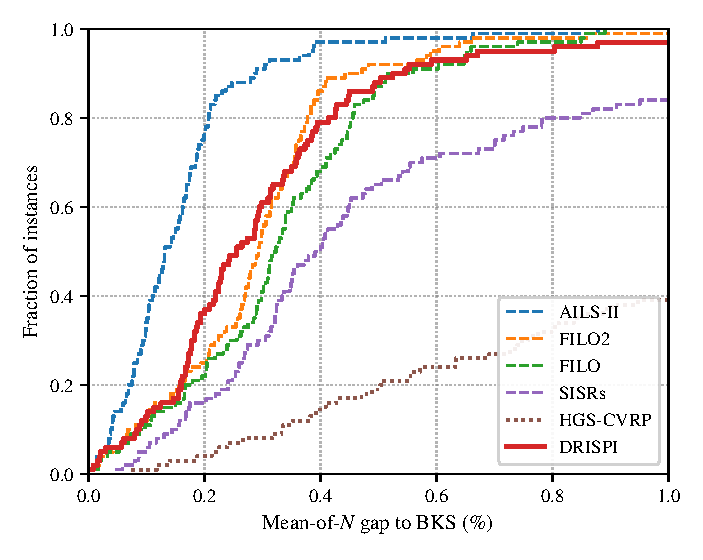
\includegraphics[width=0.8\textwidth]{figures/gap_ecdf.pdf}
\caption{Empirical CDF of the Mean-of-$N$ Gap to the Current BKS.} \label{fig:gap-ecdf}
\end{figure}

Figure~\ref{fig:gap-ecdf} shows why the Table~\ref{tab:solver-summary} means understate \gls{drispi}'s typical result and its tail at once: \gls{drispi}'s mean-of-3 gap has a mean of 0.309\% against a median of 0.255\% (interquartile range 0.172\%--0.380\%, ninetieth percentile 0.527\%, maximum 1.683\%), a right-skewed distribution in which most instances sit below the mean and a short tail sits well above it. \gls{drispi}'s curve tracks above FILO2's up to a gap of about 0.3\% (61\% of instances at or below that gap, against 55\% for FILO2) and falls below it from 0.4\% (79\% against 86\%), the crossover the non-significant paired mean-of-$N$ test against FILO2 allows: \gls{drispi} wins on the tighter half of the distribution and loses on the wider half. Against FILO, \gls{drispi}'s curve stays at or above FILO's over the range shown, consistent with the near-even 53-of-100 split in the paired test. HGS-CVRP's curve sits below all five other curves across the entire range shown: only 39\% of its instances reach a gap of one percent or less, and it does not visibly approach the other curves anywhere in the figure, consistent with the wide, significant margin the paired test above reports against it.

Table~\ref{tab:gap-tail} lists the instances behind that tail, the largest mean-of-3 gaps in Table~\ref{tab:xl-summary}, in descending order down to about $+0.6$ percent.

\begin{table}[H]
\centering
\caption{\gls{drispi}'s Largest Mean-of-3 Gap to Current \gls{bks} (Abbr. as per Section~\ref{sec:stu-dataset}).}
\label{tab:gap-tail}
\begin{tabular}{@{}lrlllrr@{}}
\toprule
Instance & $n$ & Depot & Customers & Demand & $r$ & Mean-of-3 Gap (\%) \\
\midrule
XL-n9571-k55 & 9{,}571 & R & R & Q & 174.7 & +1.68 \\
XL-n6034-k61 & 6{,}034 & R & C (5) & 5-10 & 98.9 & +1.18 \\
XL-n2634-k17 & 2{,}634 & R & C (4) & 1-10 & 162.6 & +1.17 \\
XL-n5174-k55 & 5{,}174 & C & C (6) & 1-10 & 94.1 & +0.88 \\
XL-n8207-k108 & 8{,}207 & C & C (2) & 1-10 & 75.9 & +0.80 \\
XL-n5902-k122 & 5{,}902 & E & RC (3) & Q & 48.8 & +0.67 \\
XL-n8028-k294 & 8{,}028 & C & R & Q & 27.3 & +0.65 \\
\bottomrule
\end{tabular}
\end{table}

Five of these seven instances fall in the dataset's ultra-long route band, $r \geq 50$ (Section~\ref{sec:stu-dataset}); Section~\ref{sec:stu-characteristics} takes up this concentration directly.

Two individual results do not appear in any aggregate. On XL-n4535-k1134, \gls{drispi}'s best-of-3 cost of 1,203,553 is below the initial \gls{bks} of 1,203,566 \citet{queirogaXLInstancesCapacitated2026} reported at publication. On XL-n1094-k157, \gls{drispi}'s best-of-3 cost matches both the initial and the current \gls{bks} exactly, at 112,431. Across all 100 instances, \gls{drispi}'s best-of-3 cost matches or beats AILS-II's mean-of-60 on 12 instances, listed in Table~\ref{tab:matches-beats}.

\begin{table}[H]
\centering
\caption{\gls{drispi}'s Best-of-3 Cost Matching or Beating a Published Reference.}
\label{tab:matches-beats}
\begin{tabular}{@{}lrrrl@{}}
\toprule
Instance & $r$ & \gls{drispi} Best-of-3 & Reference Cost & Reference \\
\midrule
XL-n1094-k157 & 7.8 & 112{,}431 & 112{,}431.0 & Initial \& current \gls{bks} \\
XL-n1281-k29 & 45.5 & 31{,}161 & 31{,}201.3 & AILS-II mean-of-60 \\
XL-n1328-k19 & 72.6 & 38{,}261 & 38{,}317.4 & AILS-II mean-of-60 \\
XL-n1374-k278 & 4.9 & 233{,}247 & 233{,}248.0 & AILS-II mean-of-60 \\
XL-n1654-k11 & 155.4 & 36{,}420 & 36{,}429.1 & AILS-II mean-of-60 \\
XL-n1794-k163 & 11.2 & 141{,}739 & 141{,}777.6 & AILS-II mean-of-60 \\
XL-n1981-k13 & 153.5 & 32{,}597 & 32{,}639.1 & AILS-II mean-of-60 \\
XL-n2307-k34 & 69.6 & 47{,}980 & 48{,}020.2 & AILS-II mean-of-60 \\
XL-n2727-k546 & 5.3 & 431{,}165 & 431{,}173.0 & AILS-II mean-of-60 \\
XL-n3804-k29 & 134.0 & 52{,}930 & 52{,}935.8 & AILS-II mean-of-60 \\
XL-n3888-k1010 & 4.2 & 1{,}881{,}512 & 1{,}882{,}369.0 & AILS-II mean-of-60 \\
XL-n4535-k1134 & 4.3 & 1{,}203{,}553 & 1{,}203{,}566.0 & Initial \gls{bks} \\
\bottomrule
\end{tabular}
\end{table}

\subsection{Performance by Instance Characteristics}\label{sec:stu-characteristics}
The XL instance set varies two candidate notions of scale at once: the customer count $n$ and the target average route length $r$ (Section~\ref{sec:stu-dataset}). The two are not interchangeable stand-ins for the same underlying quantity. $r$ is not derived from $n$; it is an independent design factor of the benchmark's own generation scheme, which fixes vehicle capacity $Q$ and fleet size jointly so that a minimum-route solution attains the target $r$ for whatever $n$ the instance happens to have, so the 100-instance design deliberately crosses a wide range of $r$ against a wide range of $n$ rather than letting one determine the other. For \gls{drispi} specifically, the two also act on the pipeline differently: $n$ sets how many customers decomposition has to distribute across $k$ subclusters, while $r$ sets how many stops a single vehicle round trip covers on average and, by construction, compresses the number of routes relative to customers once it grows large. A regression that treats $n$ as the only scale variable therefore risks crediting to instance size a pattern that a small number of long-route instances are actually driving.

A linear regression of the mean-of-3 gap on $n$ over all 100 instances gives a slope of \todo{NUMBER: gap-on-$n$ slope, all 100 instances} (test statistic \todo{NUMBER: gap-on-$n$ test statistic, all 100 instances}, $p = $~\todo{NUMBER: gap-on-$n$ p-value, all 100 instances}, 95\% confidence interval \todo{NUMBER: gap-on-$n$ 95\% CI, all 100 instances}). We define the long-route instances as those in the dataset's own ultra-long route band, $r \geq 50$ (Section~\ref{sec:stu-dataset}), a threshold fixed by the benchmark's band definition rather than chosen after inspecting the gaps, and it separates 14 long-route instances from the remaining 86. Restricting the same regression to those 86 instances changes the slope to \todo{NUMBER: gap-on-$n$ slope, $r<50$ only} (test statistic \todo{NUMBER: gap-on-$n$ test statistic, $r<50$ only}, $p = $~\todo{NUMBER: gap-on-$n$ p-value, $r<50$ only}, 95\% confidence interval \todo{NUMBER: gap-on-$n$ 95\% CI, $r<50$ only}). \todo{NUMBER: state here, once both p-values above are filled in, whether the $n$-slope loses significance on the $r<50$ subset}. If it does, the scale-gap relationship measured over all 100 instances is carried substantially by the 14 long-route instances rather than by instance size on its own.

This pattern is consistent with what decomposition does to a long route rather than with a direct effect of $n$. Every clustering method in Table~\ref{tab:decomp-methods} draws its partition from customer coordinates or route centroids and the dissimilarity metric of Equation~\ref{eq:decomp-dissimilarity}, without reference to which vehicle will eventually need which customers; a long route spans a customer set spread further apart on average than a short route serving a comparable number of stops, and that same spatial spread makes it more likely that some clustering cut line passes through the route rather than around it. Once a long route straddles a cluster boundary this way, the routing stage (Section~\ref{sec:fra-routing}) still solves each side of the cut to a good local optimum in isolation, but the seam between them is exactly the kind of defect BG-AILS exists to repair (Section~\ref{sec:fra-bg-ails}). BG-AILS repairs every seam in an instance under the same fixed chain length of $k$ cross-reconnects and the same wall-clock budget of Equation~\ref{eq:bg-ails-budget} regardless of how many of those seams cut through a long route rather than a short one, so an instance whose long routes cross more boundaries has more repair work competing for a budget that does not grow to match it.

Figure~\ref{fig:characteristics-panels} sets this account against the remaining instance characteristics descriptively: depot position, customer distribution, demand distribution, and $n$, each summarized by the per-category mean-of-3 gap (panels a-c) or plotted directly against the per-instance gap (panel d), rather than argued from.

\begin{figure}[H]
\centering
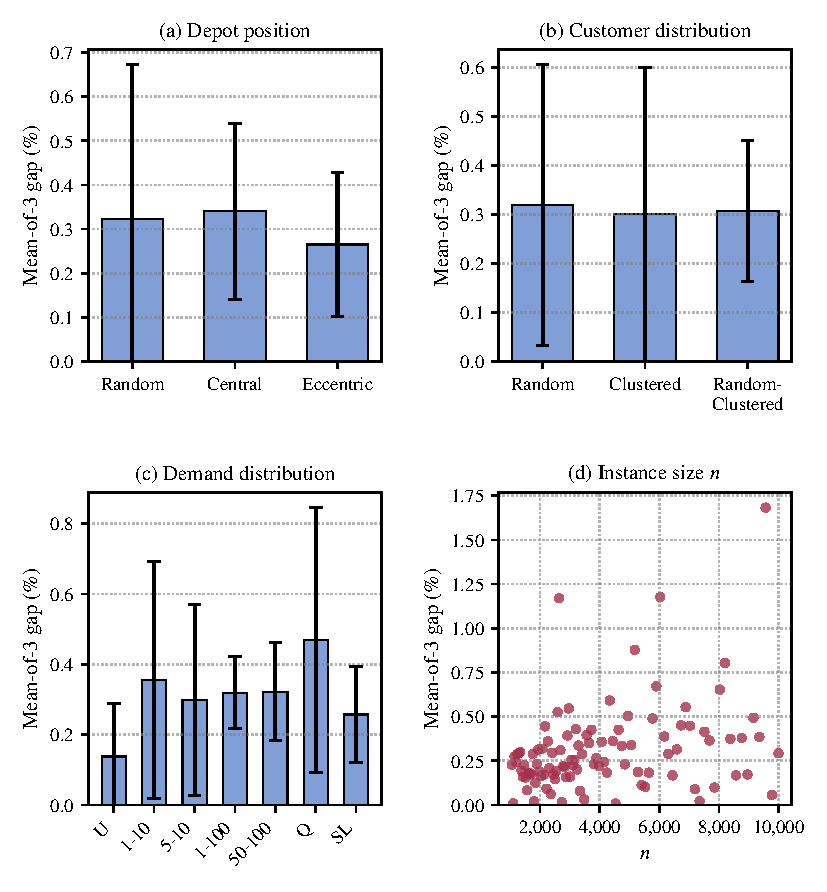
\includegraphics[width=0.85\textwidth]{figures/characteristics_panels.pdf}
\caption{Mean-of-3 Gap to the Current \gls{bks} by Instance Characteristic, Across All 100 XL instances (Error Bars Are One Sample Standard Deviation).}
\label{fig:characteristics-panels}
\end{figure}

\subsection{HAOS Weights}\label{sec:stu-haos}
Investigate how HAOS weights are converging and if there are obvious tendencies. Interpret the results. 

Are some HAOS levels converging always to the same result? Are some HAOS levels always converging in a similar way subject to the instance characteristics? Whats the variance in HAOS weight convergence? Do they differ a lot from seed to seed and are sensitive to randomness?

Are the results interpretable in general?

\subsection{Convergence Behavior}\label{sec:stu-convergence}
Show how the convergence behavior is like for \gls{drispi} by wallclock time and iterations. Use this chapter to also investigate improvement sources (quantitatively and qualitatively).
\chapter{Conclusion}\label{chapter:conclusion}
Short introduction. It should relect on the primary and secondary research questions.

\section{Highlights}\label{sec:con-highlights}
Mention the strengths (such as adaptiveness through online learning) and weaknesses (such as more CPU time required) of the framework.

Also elaborate on the main contributions of the thesis.

\section{Limitations}\label{sec:con-limitations}

% --- 1. Hardware ----------------------------------------------------------
Table~\ref{tab:solver-summary} compares runs that differ in hardware, parallelism, and total budget,
and none of its gaps correct for these differences. \citet{queirogaXLInstancesCapacitated2026} ran
every published solver on a single thread of a machine with two AMD EPYC~9654
processors (Zen~4, 2.40\,GHz), 60~seeds of two hours per instance. \gls{drispi} ran
three seeds of two hours per instance on eight pinned cores of two Intel Xeon
Platinum 8280L processors (Cascade Lake, 2.70\,GHz; Section~\ref{sec:stu-implementation}). Both machines were
shared: the published runs executed as up to 50 parallel jobs on one machine,
\gls{drispi} as six concurrent containers, three per socket, pinned to physical cores.

\citet{accorsiGuidelinesComputationalTesting2022} recommend bringing running times from different processors
to a common scale with the PassMark single-thread rating before comparing them.
The EPYC~9654 rates 2,898\footnote{\url{https://www.cpubenchmark.net/cpu.php?cpu=AMD+EPYC+9654&id=5088}, accessed September 19, 2026.} and the Platinum 8280L 2,316\footnote{\url{https://www.cpubenchmark.net/cpu.php?cpu=Intel+Xeon+Platinum+8280L+@+2.70GHz&id=6729}, accessed September 19, 2026.}, a factor of 1.25. That factor is a lower bound: the 8280L rating rests on few samples and is measured at the 4.0\,GHz single-core turbo, which the chip cannot hold with 24 of its 28 cores busy. Scaled this way, \gls{drispi}'s 7,200 seconds
per run correspond to at most 5,800 seconds on the published solvers' processor,
per core. Table~\ref{tab:solver-summary} reports unscaled gaps: \gls{drispi} was not rerun with a longer
limit to offset the slower hardware, and a single-thread rating says nothing
about how well eight cores are used in parallel.

% --- 2. Budget: mean vs best ------------------------------------------------
The budget asymmetry points in opposite directions for the two columns of
Table~\ref{tab:solver-summary}. Per run, \gls{drispi} used 16 core-hours (at most 12.8 after PassMark scaling)
against two CPU-hours for each published run, so the mean-of-$N$ column compares runs in which \gls{drispi} had eight
times the cores, on older hardware. Those eight cores do not deliver eight times
the search. Subcluster routing runs in waves that leave \texttt{dri} cores idle
whenever the last wave holds fewer than six subclusters, the main loop blocks
while it waits for BG-AILS (Figure~\ref{fig:pipeline-swimlane}), and three containers share the memory
bandwidth and last-level cache of each socket.
% TODO: quantify if you have it (e.g. mean dri core utilization per iteration).
Per instance, the relation reverses. A published best-of-60 draws on 120 CPU-hours
and 120 hours of wall-clock time, \gls{drispi}'s best-of-3 on 48 core-hours (at most 38
after PassMark scaling) and six hours. The minimum of 60 runs from a distribution lies systematically below the
minimum of three, so the best-of-$N$ column favors the published solvers by
construction. Neither column is an equal-resource ranking.

% --- 3. Run length and HAOS convergence ------------------------------------
The 7,200-second limit matches the published per-run budget, not the run length
\gls{drispi} needs. HAOS learns online. For the first ten iterations it draws uniformly
and updates nothing (Section~3.1), and after that every draw of a weak arm still
costs a full decomposition, routing, and BG-AILS pass. Under a fixed wall-clock
limit, the number of completed iterations therefore bounds how far the wheels can
move. That bound is tightest where one routing wave is expensive: large $n$ and,
separately, long routes. Section~\ref{sec:stu-convergence} reports the realized iteration counts and
[TODO: share of runs still improving in the final 20 minutes]. Whether a longer
run would close the remaining gap on these instances was not tested.

% --- 4. Statistical resolution (S = 3) ---------------------------------------
$S = 3$ was sized for the grand mean $\bar{G}$ (Section~\ref{sec:stu-repetitions}) and supports claims
at that level only. The forecast 95\% half-width of $\bar{G}$ is 0.013\,pp. For a
single instance, the mean of three seeds at the pilot standard deviation of
0.118\,pp has a standard error of 0.068\,pp and, with two degrees of freedom
($t_{0.975,2} = 4.30$), a 95\% half-width of about 0.29\,pp. That is more than
twenty times wider, and wider still on the high-variance instances. The
per-instance results in Section~\ref{sec:stu-results} (the largest gaps in Table~\ref{tab:gap-tail}, the instances
where \gls{drispi}'s best-of-3 matches or beats a published result in Table~\ref{tab:matches-beats}, and
[TODO: small subgroups in Section~\ref{sec:stu-characteristics}]) are therefore descriptive. Across
100 instances, some differences of that size will arise from the seed alone.

The seed term is also not the largest source of error. Two pilot campaigns that
differed only in execution environment showed a batch effect of about 0.039\,pp,
three times the $S = 3$ half-width, and more seeds would not have reduced it.
Shared-server load and Docker pinning are part of the measurement rather than a
nuisance the design controlled.

% --- 5. No fixed-configuration control arm ----------------------------------
The contribution of HAOS is established descriptively, through the weight
trajectories of Section~\ref{sec:stu-haos}, and not against a control arm that freezes the draw
at one configuration for the whole run under the same budget. That arm was not
run. The 300-run campaign behind Section~\ref{sec:stu-comparison} used the server allocation
available for this thesis, and a controlled comparison needs a full campaign run
alongside it; a subset carved out of the existing allocation would confound the
two. \citet{altendeiteringDRSCICVRP2026} leave the same gap for DRSCI, a \gls{drispi}
predecessor that draws paradigm, $k$, and solver uniformly at random each
iteration without learning. Whether HAOS pays a sampling cost relative to a single
committed configuration, or improves on it, remains open.

\section{Future Research}\label{sec:con-future}
Use the HAOS weights to train an offline learning model and inject the results back into the framework. This effectively eliminates the warm-up period and will lead to a substential speed-up of the framework.

Also mention that the framework, other than monolithic solvers, is highly adaptable to different instances and VRP variants. Since it only requires the plug-and-play of capable clustering methods and solvers on the their respective stages.
%\include{chapters/Chapter2}
%...include other chapters here
\bibliography{bibliography/literature}
\part*{Appendix}
\addcontentsline{toc}{chapter}{Appendix}
\setcounter{section}{0}
\renewcommand{\thesection}{\arabic{section}}
\renewcommand{\theHsection}{A.\arabic{section}}
\renewcommand{\theequation}{\arabic{equation}}
\setcounter{table}{0}
\renewcommand{\thetable}{A.\arabic{table}}
\renewcommand{\theHtable}{A.\arabic{table}}
\setcounter{figure}{0}
\renewcommand{\thefigure}{A.\arabic{figure}}
\renewcommand{\theHfigure}{A.\arabic{figure}}
\section{Set Covering Formulation}\label{app:set-covering}
Section~\ref{sec:fra-sp} introduces set covering (SC) as the fallback \gls{drispi} runs in place of set partitioning (SP) when the route pool does not yet cover every customer at least a minimum number of times. With $R$ the route pool at the time of the solve, $c_r$ the cost of route $r \in R$, $C$ the customer set of the instance (Section~\ref{sec:lit-problem}), $C_r \subseteq C$ the customer set of route $r$, and $x_r \in \{0, 1\}$ selecting route $r$, SC relaxes the partition equality of SP (Equation~\ref{eq:sp-partition}) to the cover inequality of \citet{garfinkelSetPartitioningProblemSetCovering1969}, who characterize set partitioning as set covering under an equality constraint:
\begin{align}
\text{min} \quad & \sum_{\mathclap{r \in R}} c_r x_r \label{eq:sc-obj}\\
\text{s.t.} \quad & \sum_{\mathclap{r \in R:\, i \in C_r}} x_r \geq 1, && \forall i \in C \label{eq:sc-cover}\\
& x_r \in \{0, 1\}, && \forall r \in R. \label{eq:sc-binary}
\end{align}
As with SP, \gls{drispi} solves the LP relaxation of Equation~\ref{eq:sc-binary}, $x_r \in [0, 1]$, first; the resulting fractional weights update the pool's quality scores in the same way regardless of whether the solve ends up running SC or SP, and the binary re-solve is warm-started from that relaxation.
\newpage
\section{XL Instance Detailed Results}\label{app:xl-results}
Table~\ref{tab:xl-summary} reports the per-instance detail underlying the Section~\ref{sec:stu-comparison} comparison: instance characteristics, \gls{drispi}'s best cost and gap to the current \gls{bks} for all 100 XL instances, alongside the initial-\gls{bks} and current-\gls{bks} reference costs.

% TODO(style): deviates from the "no shrinking below body size" rule in
% STYLE.md \S8; kept in portrait (rather than the rotating/sidewaystable
% default for wide tables) at the user's request, which requires scriptsize
% to fit twelve columns inside \textwidth.
\begin{scriptsize}
\setkomafont{caption}{\normalsize}
\setkomafont{captionlabel}{\normalsize}
\setlength{\tabcolsep}{3pt}
\begin{longtable}{@{}rlcllrrrrrrr@{}}
\caption{Instance-Level Best-of-3 Results for \gls{drispi} on the 100 XL Instances.}\label{tab:xl-summary}\\
\toprule
& & & & & & & \multicolumn{2}{c}{\gls{drispi}} & \multicolumn{2}{c}{Initial BKS} & \multicolumn{1}{c}{BKS} \\
\cmidrule(lr){8-9} \cmidrule(lr){10-11} \cmidrule(lr){12-12}
\# & Name & Dep & Cust & Dem & $Q$ & $r$ & \multicolumn{1}{c}{Cost} & Gap (\%) & \multicolumn{1}{c}{Cost} & Gap (\%) & \multicolumn{1}{c}{Cost} \\
\midrule
\endfirsthead
\multicolumn{12}{c}{\tablename\ \thetable{} -- continued from previous page}\\
\toprule
& & & & & & & \multicolumn{2}{c}{\gls{drispi}} & \multicolumn{2}{c}{Initial BKS} & \multicolumn{1}{c}{BKS} \\
\cmidrule(lr){8-9} \cmidrule(lr){10-11} \cmidrule(lr){12-12}
\# & Name & Dep & Cust & Dem & $Q$ & $r$ & \multicolumn{1}{c}{Cost} & Gap (\%) & \multicolumn{1}{c}{Cost} & Gap (\%) & \multicolumn{1}{c}{Cost} \\
\midrule
\endhead
\bottomrule
\endfoot
\bottomrule
\endlastfoot
1 & XL-n1048-k237 & E & R & SL & 128 & 4.7 & 380{,}637 & +0.14 & 380{,}211 & +0.03 & 380{,}107 \\
2 & XL-n1094-k157 & C & C (6) & U & 7 & 7.8 & 112{,}441 & +0.01 & 112{,}431 & +0.00 & 112{,}431 \\
3 & XL-n1141-k112 & R & RC (3) & 50-100 & 761 & 10.2 & 95{,}849 & +0.22 & 95{,}727 & +0.09 & 95{,}638 \\
4 & XL-n1188-k96 & R & RC (3) & Q & 782 & 12.4 & 104{,}590 & +0.18 & 104{,}415 & +0.01 & 104{,}402 \\
5 & XL-n1234-k55 & E & R & 1-10 & 126 & 22.7 & 96{,}809 & +0.21 & 96{,}647 & +0.05 & 96{,}603 \\
6 & XL-n1281-k29 & C & C (5) & 1-100 & 2267 & 45.5 & 31{,}168 & +0.27 & 31{,}101 & +0.06 & 31{,}083 \\
7 & XL-n1328-k19 & R & RC (3) & 5-10 & 542 & 72.6 & 38{,}288 & +0.23 & 38{,}247 & +0.12 & 38{,}201 \\
8 & XL-n1374-k278 & C & R & Q & 248 & 4.9 & 233{,}360 & +0.18 & 233{,}049 & +0.05 & 232{,}940 \\
9 & XL-n1421-k232 & E & C (4) & 1-100 & 309 & 6.1 & 385{,}216 & +0.15 & 384{,}826 & +0.05 & 384{,}646 \\
10 & XL-n1468-k151 & E & R & 50-100 & 726 & 9.7 & 250{,}506 & +0.19 & 250{,}166 & +0.06 & 250{,}028 \\
11 & XL-n1514-k106 & C & RC (4) & 5-10 & 107 & 14.2 & 92{,}468 & +0.08 & 92{,}425 & +0.03 & 92{,}398 \\
12 & XL-n1561-k75 & R & C (4) & U & 21 & 21.9 & 101{,}593 & +0.05 & 101{,}549 & +0.01 & 101{,}540 \\
13 & XL-n1608-k39 & C & RC (3) & SL & 337 & 42.1 & 48{,}075 & +0.14 & 48{,}021 & +0.02 & 48{,}009 \\
14 & XL-n1654-k11 & E & R & 1-10 & 845 & 155.4 & 36{,}420 & +0.14 & 36{,}385 & +0.04 & 36{,}370 \\
15 & XL-n1701-k562 & R & C (6) & 50-100 & 227 & 3.0 & 521{,}696 & +0.16 & 521{,}136 & +0.06 & 520{,}843 \\
16 & XL-n1748-k271 & R & C (3) & Q & 270 & 6.4 & 174{,}166 & +0.23 & 173{,}896 & +0.08 & 173{,}759 \\
17 & XL-n1794-k163 & C & R & U & 11 & 11.2 & 141{,}732 & +0.01 & 141{,}729 & +0.00 & 141{,}724 \\
18 & XL-n1841-k126 & E & RC (2) & SL & 186 & 14.6 & 214{,}193 & +0.10 & 214{,}038 & +0.03 & 213{,}981 \\
19 & XL-n1888-k82 & E & R & 5-10 & 173 & 23.1 & 143{,}852 & +0.20 & 143{,}623 & +0.05 & 143{,}558 \\
20 & XL-n1934-k46 & C & C (6) & 1-100 & 2166 & 42.2 & 53{,}118 & +0.26 & 53{,}013 & +0.06 & 52{,}980 \\
21 & XL-n1981-k13 & R & RC (2) & 1-10 & 832 & 153.5 & 32{,}638 & +0.28 & 32{,}580 & +0.10 & 32{,}546 \\
22 & XL-n2028-k617 & C & C (6) & 50-100 & 247 & 3.3 & 544{,}872 & +0.13 & 544{,}403 & +0.04 & 544{,}166 \\
23 & XL-n2074-k264 & E & R & 1-100 & 401 & 7.8 & 422{,}390 & +0.27 & 421{,}627 & +0.09 & 421{,}250 \\
24 & XL-n2121-k186 & R & RC (5) & 1-10 & 62 & 11.4 & 283{,}450 & +0.12 & 283{,}211 & +0.04 & 283{,}105 \\
25 & XL-n2168-k138 & C & R & Q & 800 & 15.7 & 127{,}607 & +0.31 & 127{,}298 & +0.07 & 127{,}210 \\
26 & XL-n2214-k131 & R & C (5) & U & 17 & 17.8 & 154{,}761 & +0.07 & 154{,}676 & +0.02 & 154{,}652 \\
27 & XL-n2261-k54 & E & RC (5) & 5-10 & 319 & 42.5 & 99{,}161 & +0.34 & 98{,}907 & +0.08 & 98{,}826 \\
28 & XL-n2307-k34 & C & R & SL & 479 & 69.6 & 48{,}015 & +0.16 & 47{,}958 & +0.05 & 47{,}936 \\
29 & XL-n2354-k631 & E & C (4) & 5-10 & 28 & 3.7 & 941{,}098 & +0.05 & 940{,}825 & +0.02 & 940{,}634 \\
30 & XL-n2401-k408 & R & RC (4) & Q & 303 & 5.9 & 464{,}192 & +0.24 & 463{,}473 & +0.08 & 463{,}084 \\
31 & XL-n2447-k290 & C & RC (2) & SL & 150 & 8.4 & 219{,}024 & +0.18 & 218{,}706 & +0.03 & 218{,}633 \\
32 & XL-n2494-k194 & E & C (2) & 1-100 & 661 & 12.9 & 361{,}485 & +0.12 & 361{,}205 & +0.04 & 361{,}057 \\
33 & XL-n2541-k121 & R & R & U & 21 & 21.7 & 146{,}515 & +0.12 & 146{,}390 & +0.03 & 146{,}345 \\
34 & XL-n2587-k66 & C & R & 50-100 & 2986 & 39.6 & 73{,}592 & +0.46 & 73{,}394 & +0.19 & 73{,}254 \\
35 & XL-n2634-k17 & R & C (4) & 1-10 & 898 & 162.6 & 31{,}909 & +0.92 & 31{,}641 & +0.07 & 31{,}619 \\
36 & XL-n2681-k540 & E & RC (3) & 1-100 & 251 & 5.0 & 799{,}847 & +0.24 & 798{,}603 & +0.09 & 797{,}906 \\
37 & XL-n2727-k546 & C & RC (5) & U & 5 & 5.3 & 431{,}171 & +0.01 & 431{,}134 & +0.01 & 431{,}108 \\
38 & XL-n2774-k286 & E & C (5) & 50-100 & 731 & 9.7 & 408{,}424 & +0.20 & 407{,}847 & +0.06 & 407{,}617 \\
39 & XL-n2821-k208 & R & R & SL & 179 & 13.5 & 217{,}118 & +0.23 & 216{,}763 & +0.07 & 216{,}622 \\
40 & XL-n2867-k120 & R & C (4) & 5-10 & 180 & 23.9 & 166{,}172 & +0.15 & 165{,}990 & +0.04 & 165{,}916 \\
41 & XL-n2914-k95 & C & RC (3) & Q & 1663 & 30.8 & 89{,}238 & +0.38 & 88{,}990 & +0.10 & 88{,}902 \\
42 & XL-n2961-k55 & E & R & 1-10 & 297 & 53.8 & 108{,}416 & +0.44 & 108{,}084 & +0.13 & 107{,}945 \\
43 & XL-n3007-k658 & C & R & 1-10 & 25 & 4.4 & 522{,}857 & +0.14 & 522{,}319 & +0.04 & 522{,}126 \\
44 & XL-n3054-k461 & E & RC (4) & 50-100 & 497 & 6.6 & 783{,}840 & +0.21 & 782{,}739 & +0.07 & 782{,}194 \\
45 & XL-n3101-k311 & R & C (3) & SL & 159 & 10.0 & 246{,}245 & +0.19 & 245{,}937 & +0.07 & 245{,}766 \\
46 & XL-n3147-k232 & R & RC (6) & 5-10 & 102 & 13.6 & 257{,}010 & +0.23 & 256{,}626 & +0.08 & 256{,}417 \\
47 & XL-n3194-k161 & C & R & Q & 1012 & 19.9 & 149{,}190 & +0.40 & 148{,}728 & +0.09 & 148{,}596 \\
48 & XL-n3241-k115 & E & C (4) & 1-100 & 1404 & 28.3 & 221{,}674 & +0.19 & 221{,}370 & +0.05 & 221{,}249 \\
49 & XL-n3287-k30 & C & C (2) & U & 111 & 112.0 & 40{,}288 & +0.24 & 40{,}229 & +0.10 & 40{,}190 \\
50 & XL-n3334-k934 & E & R & 1-10 & 20 & 3.5 & 1{,}453{,}192 & +0.06 & 1{,}452{,}698 & +0.02 & 1{,}452{,}353 \\
51 & XL-n3408-k524 & R & RC (3) & Q & 353 & 6.5 & 679{,}708 & +0.25 & 678{,}643 & +0.09 & 678{,}024 \\
52 & XL-n3484-k436 & E & C (6) & U & 8 & 8.2 & 703{,}472 & +0.02 & 703{,}355 & +0.01 & 703{,}319 \\
53 & XL-n3561-k229 & C & RC (5) & 1-100 & 779 & 15.6 & 209{,}939 & +0.36 & 209{,}386 & +0.09 & 209{,}191 \\
54 & XL-n3640-k211 & R & R & 5-10 & 130 & 17.2 & 190{,}159 & +0.33 & 189{,}724 & +0.10 & 189{,}531 \\
55 & XL-n3721-k77 & E & RC (2) & SL & 371 & 48.8 & 163{,}195 & +0.35 & 162{,}862 & +0.14 & 162{,}630 \\
56 & XL-n3804-k29 & C & R & 50-100 & 10064 & 134.0 & 52{,}924 & +0.16 & 52{,}885 & +0.09 & 52{,}838 \\
57 & XL-n3888-k1010 & R & C (2) & SL & 128 & 4.2 & 1{,}880{,}215 & +0.16 & 1{,}880{,}368 & +0.17 & 1{,}877{,}119 \\
58 & XL-n3975-k687 & C & RC (4) & 1-10 & 32 & 5.6 & 526{,}535 & +0.19 & 525{,}901 & +0.06 & 525{,}560 \\
59 & XL-n4063-k347 & E & R & Q & 598 & 11.7 & 549{,}989 & +0.30 & 548{,}931 & +0.11 & 548{,}330 \\
60 & XL-n4153-k291 & R & C (3) & 1-100 & 726 & 14.3 & 356{,}513 & +0.21 & 356{,}034 & +0.07 & 355{,}780 \\
61 & XL-n4245-k203 & R & R & U & 21 & 21.0 & 229{,}846 & +0.14 & 229{,}659 & +0.06 & 229{,}521 \\
62 & XL-n4340-k148 & E & RC (6) & 50-100 & 2204 & 29.3 & 245{,}007 & +0.46 & 244{,}226 & +0.14 & 243{,}895 \\
63 & XL-n4436-k48 & C & C (4) & 5-10 & 706 & 94.1 & 61{,}607 & +0.29 & 61{,}477 & +0.07 & 61{,}431 \\
64 & XL-n4535-k1134 & R & C (4) & U & 4 & 4.3 & 1{,}203{,}629 & +0.01 & 1{,}203{,}566 & +0.00 & 1{,}203{,}512 \\
65 & XL-n4635-k790 & C & RC (4) & 1-100 & 294 & 5.9 & 612{,}416 & +0.44 & 610{,}650 & +0.15 & 609{,}734 \\
66 & XL-n4738-k487 & E & R & Q & 499 & 9.7 & 762{,}178 & +0.33 & 760{,}501 & +0.11 & 759{,}649 \\
67 & XL-n4844-k321 & R & R & SL & 188 & 15.1 & 405{,}362 & +0.23 & 404{,}652 & +0.06 & 404{,}429 \\
68 & XL-n4951-k203 & E & RC (5) & 50-100 & 1848 & 24.5 & 286{,}057 & +0.45 & 285{,}269 & +0.18 & 284{,}769 \\
69 & XL-n5061-k184 & C & C (5) & 5-10 & 206 & 27.4 & 161{,}994 & +0.32 & 161{,}629 & +0.09 & 161{,}480 \\
70 & XL-n5174-k55 & C & C (6) & 1-10 & 520 & 94.1 & 61{,}712 & +0.75 & 61{,}382 & +0.21 & 61{,}254 \\
71 & XL-n5288-k1246 & E & R & 50-100 & 318 & 4.2 & 1{,}961{,}862 & +0.19 & 1{,}960{,}101 & +0.10 & 1{,}958{,}205 \\
72 & XL-n5406-k783 & R & RC (2) & 1-10 & 38 & 6.8 & 1{,}041{,}298 & +0.11 & 1{,}040{,}536 & +0.04 & 1{,}040{,}141 \\
73 & XL-n5526-k553 & R & C (3) & U & 10 & 10.0 & 337{,}149 & +0.09 & 336{,}898 & +0.02 & 336{,}843 \\
74 & XL-n5649-k401 & E & R & SL & 181 & 14.1 & 645{,}479 & +0.14 & 644{,}866 & +0.05 & 644{,}562 \\
75 & XL-n5774-k290 & C & RC (4) & 1-100 & 1012 & 19.9 & 250{,}921 & +0.41 & 250{,}207 & +0.12 & 249{,}895 \\
76 & XL-n5902-k122 & E & RC (3) & Q & 2663 & 48.8 & 218{,}452 & +0.66 & 217{,}447 & +0.20 & 217{,}012 \\
77 & XL-n6034-k61 & R & C (5) & 5-10 & 744 & 98.9 & 64{,}812 & +0.87 & 64{,}448 & +0.31 & 64{,}251 \\
78 & XL-n6168-k1922 & C & R & 1-100 & 162 & 3.2 & 1{,}532{,}658 & +0.34 & 1{,}530{,}010 & +0.17 & 1{,}527{,}390 \\
79 & XL-n6305-k1042 & R & RC (2) & Q & 268 & 6.0 & 1{,}179{,}538 & +0.30 & 1{,}177{,}528 & +0.13 & 1{,}176{,}002 \\
80 & XL-n6445-k628 & E & R & 5-10 & 77 & 10.2 & 997{,}627 & +0.15 & 996{,}623 & +0.05 & 996{,}117 \\
81 & XL-n6588-k473 & C & C (4) & 1-10 & 76 & 13.8 & 334{,}693 & +0.26 & 334{,}068 & +0.07 & 333{,}822 \\
82 & XL-n6734-k330 & R & RC (2) & 50-100 & 1534 & 20.4 & 449{,}068 & +0.35 & 448{,}031 & +0.12 & 447{,}486 \\
83 & XL-n6884-k148 & E & C (4) & SL & 357 & 46.4 & 182{,}403 & +0.45 & 181{,}809 & +0.12 & 181{,}585 \\
84 & XL-n7037-k38 & C & R & U & 187 & 187.1 & 71{,}041 & +0.40 & 70{,}845 & +0.12 & 70{,}760 \\
85 & XL-n7193-k1683 & E & RC (2) & 5-10 & 32 & 4.2 & 2{,}960{,}255 & +0.07 & 2{,}958{,}979 & +0.03 & 2{,}958{,}205 \\
86 & XL-n7353-k1471 & R & R & U & 5 & 5.1 & 1{,}538{,}039 & +0.02 & 1{,}537{,}811 & +0.01 & 1{,}537{,}702 \\
87 & XL-n7516-k859 & C & C (2) & 1-100 & 439 & 8.8 & 575{,}265 & +0.40 & 573{,}902 & +0.16 & 572{,}984 \\
88 & XL-n7683-k602 & R & RC (3) & 50-100 & 957 & 12.8 & 703{,}772 & +0.37 & 702{,}098 & +0.14 & 701{,}151 \\
89 & XL-n7854-k365 & E & C (2) & SL & 223 & 21.5 & 659{,}532 & +0.07 & 659{,}221 & +0.02 & 659{,}075 \\
90 & XL-n8028-k294 & C & R & Q & 1386 & 27.3 & 267{,}870 & +0.59 & 266{,}900 & +0.23 & 266{,}295 \\
91 & XL-n8207-k108 & C & C (2) & 1-10 & 415 & 75.9 & 118{,}748 & +0.59 & 118{,}274 & +0.19 & 118{,}050 \\
92 & XL-n8389-k2028 & E & RC (4) & 1-100 & 208 & 4.1 & 3{,}364{,}681 & +0.34 & 3{,}358{,}731 & +0.16 & 3{,}353{,}305 \\
93 & XL-n8575-k1297 & R & R & 1-10 & 36 & 6.5 & 1{,}089{,}997 & +0.15 & 1{,}089{,}137 & +0.07 & 1{,}088{,}376 \\
94 & XL-n8766-k1032 & R & RC (4) & 50-100 & 637 & 8.5 & 907{,}882 & +0.31 & 906{,}406 & +0.15 & 905{,}060 \\
95 & XL-n8960-k634 & E & C (5) & 5-10 & 106 & 14.1 & 774{,}077 & +0.15 & 773{,}383 & +0.06 & 772{,}906 \\
96 & XL-n9160-k379 & C & R & SL & 237 & 24.2 & 325{,}176 & +0.49 & 324{,}092 & +0.15 & 323{,}596 \\
97 & XL-n9363-k209 & C & RC (2) & U & 45 & 45.2 & 205{,}962 & +0.29 & 205{,}575 & +0.10 & 205{,}369 \\
98 & XL-n9571-k55 & R & R & Q & 8773 & 174.7 & 107{,}910 & +1.47 & 106{,}791 & +0.42 & 106{,}344 \\
99 & XL-n9784-k2774 & E & C (4) & 1-10 & 19 & 3.4 & 4{,}078{,}970 & +0.05 & 4{,}078{,}217 & +0.03 & 4{,}076{,}936 \\
100 & XL-n10001-k1570 & E & RC (2) & 50-100 & 479 & 6.4 & 2{,}337{,}368 & +0.29 & 2{,}333{,}757 & +0.13 & 2{,}330{,}666 \\

\end{longtable}
\end{scriptsize}

\section{HAOS Weight Diagnostics}\label{app:haos-diagnostics}
The figures in this appendix support Section~\ref{sec:results-haos}. They are not part of the argument in the body: the $k$-share heatmap and the top-arm share describe where the wheels finished, and the three diagnostic panels record the weight range, the time spent on the decay floor, and the gap between the observed weight and the interior fixed point of the recurrence.

\begin{figure}[H]
\centering
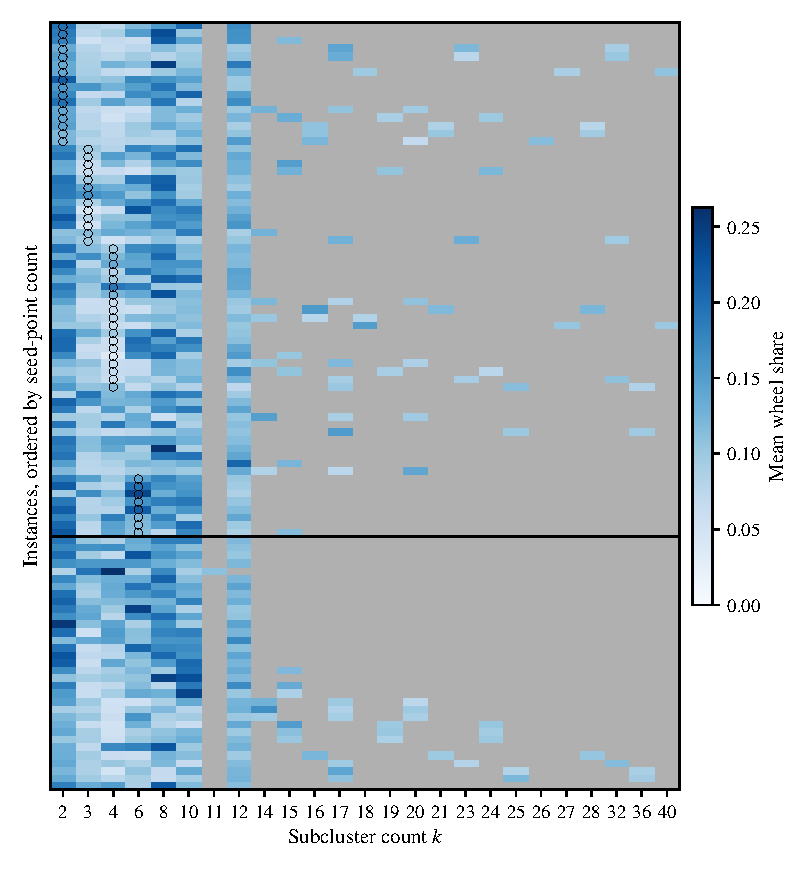
\includegraphics[width=\textwidth]{figures/haos_k_heatmap.pdf}
\caption{Final $k$-Wheel Share, Averaged over the Three Seeds, Supporting Section~\ref{sec:results-haos}. Rows are the 100 XL instances, ordered by the number of customer seed points used to generate them; the random instances, which have none, form the block below the horizontal line. Open circles mark the cell where $k$ equals that seed-point count. Colour runs from zero to the largest share in the figure. Grey cells are arms outside that instance's $k$ domain.}
\label{fig:haos-k}
\end{figure}

\begin{figure}[H]
\centering
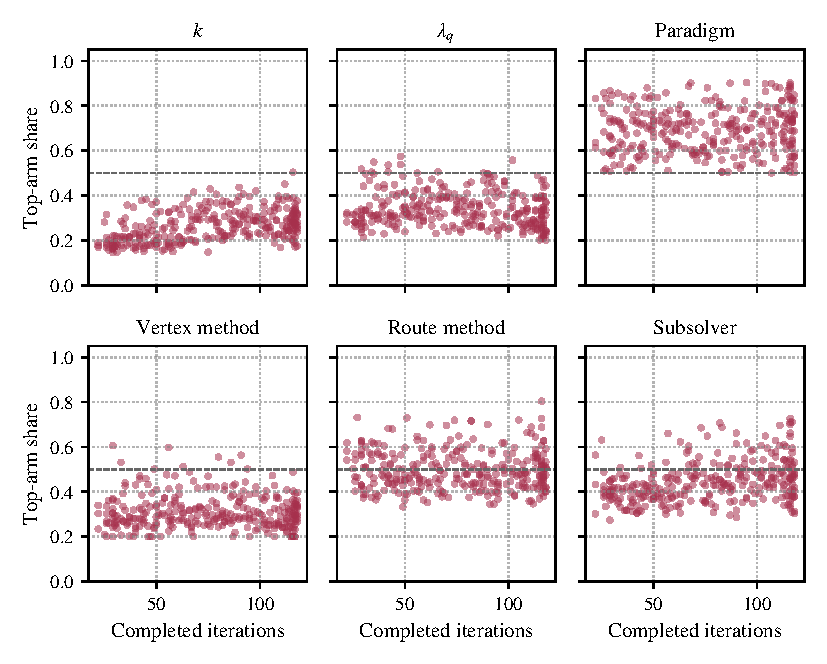
\includegraphics[width=\textwidth]{figures/haos_top_arm.pdf}
\caption{Top-Arm Share of Each HAOS Wheel Against Completed \gls{dri} Iterations, Supporting Section~\ref{sec:results-haos}. The dashed line is a share of one half. A two-arm wheel lies on or above that line on every draw.}
\label{fig:haos-toparm}
\end{figure}

\begin{figure}[H]
\centering
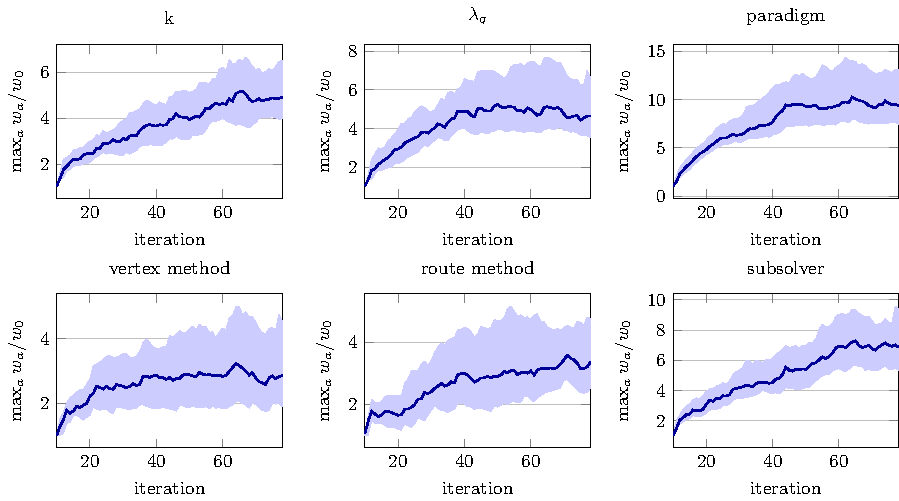
\includegraphics[width=\textwidth]{figures/haos_diag_weight_range.pdf}
\caption{Weight Range of the Six Wheels Against Iteration, Supporting Section~\ref{sec:results-haos}. The curve is the median ratio of the largest weight to $w_0$, and the band is the interquartile range.}
\label{fig:haos-weight-range}
\end{figure}

\begin{figure}[H]
\centering
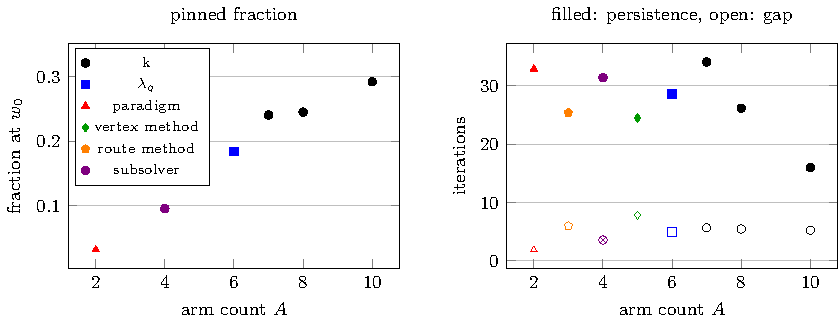
\includegraphics[width=\textwidth]{figures/haos_diag_pinned.pdf}
\caption{Decay-Floor Occupancy and Spell Length, Supporting Section~\ref{sec:results-haos}. The left panel is the fraction of post-warm-up snapshots sitting on the floor. The right panel is the mean spell above the floor and the mean gap before the arm is drawn again.}
\label{fig:haos-pinned}
\end{figure}

\begin{figure}[H]
\centering
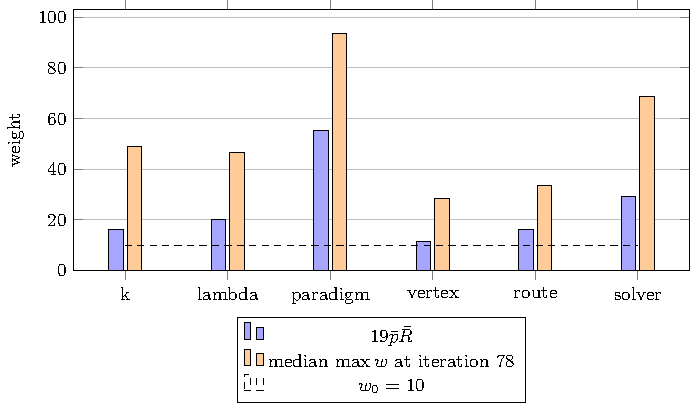
\includegraphics[width=0.92\textwidth]{figures/haos_diag_equilibrium.pdf}
\caption{Observed Median Maximum Weight Against the Interior Fixed Point $19\bar{p}\bar{R}$, Supporting Section~\ref{sec:results-haos}.}
\label{fig:haos-equilibrium}
\end{figure}
\cleardoublepage
\newgeometry{left=20mm,right=20mm,top=20mm,bottom=10mm}
\thispagestyle{empty}
\changefont{phv}{m}{n}
\textbf{Declaration Of Authorship}\\

I hereby solemnly declare that I have completed the present work independently. All ideas taken directly or indirectly from external sources have been clearly identified as such.

I am aware that the work may be examined in digital form to determine whether unauthorized aids were used and whether it constitutes - either in whole or in part - plagiarism. For the purpose of comparison with existing sources, my work may be entered into a database and, after review, may remain there for comparison with future submissions. No further reproduction or usage rights are thereby granted. This work has neither been submitted to another examination authority nor published.


\vspace{2cm}
Place, Date
\vspace{2cm}

Lucca Altendeitering
\cleardoublepage
\newgeometry{left=20mm,right=20mm,top=20mm,bottom=10mm}
\thispagestyle{empty}
\changefont{phv}{m}{n}
\textbf{Declaration of AI Use}\\

Download the \href{https://www.ot.mgt.tum.de/fileadmin/w00cjr/log/Theses_ProjectStudies/Logscm_AI_Declaration.pdf}{Declaration of AI Use} from the website, complete it truthfully, and include it as a separate page at the end of your final thesis PDF here instead of this page.

\end{document}